% LaTeX Generic essay template
% Copyright (C) 2017  Shen Zhou Hong <shen@hong.io>
%
% This program is free software: you can redistribute it and/or modify
% it under the terms of the GNU General Public License as published by
% the Free Software Foundation, either version 3 of the License, or
% (at your option) any later version.
%
% This program is distributed in the hope that it will be useful,
% but WITHOUT ANY WARRANTY; without even the implied warranty of
% MERCHANTABILITY or FITNESS FOR A PARTICULAR PURPOSE.  See the
% GNU General Public License for more details.
%
% You should have received a copy of the GNU General Public License
% along with this program.  If not, see <https://www.gnu.org/licenses/>.

% For more information on documentclass configuration, see:
% https://texblog.org/2013/02/13/latex-documentclass-options-illustrated/#formula
\documentclass[
  10pt,
  a4paper,
  protrudelabels,
  onehalfspacing,
  extraligatures,
  titlepage,
  english,
  widemargins,
  oneside
]{humanize}

% Configuration for 'fancy' headers and footers
\usepackage{fancyhdr}               % For fancy headings
\usepackage{lastpage}               % Gives us \lastpage
% Settings used by \usepackage{fancyhdr}
\fancypagestyle{plain}{
  % Clear all definitions from the fancy pagestyle
  \fancyhf{}
  \renewcommand{\headrulewidth}{0pt}
  \renewcommand{\footrulewidth}{0pt}

  % Ensure page numbers are the form page n of m.
  \fancyfoot[C]{Page~\thepage~of~\pageref*{LastPage}}
}
\fancypagestyle{fancy}{
  % Fancy Header Formatting
  \renewcommand{\headrulewidth}{0.4pt}
  \fancyhead[L]{Final Project}
  \fancyhead[C]{}
  \fancyhead[R]{Goldsmiths, University of London}

  % Fancy Footer Formatting
  \renewcommand{\footrulewidth}{0pt}
  \fancyfoot[L]{}
  \fancyfoot[C]{Page~\thepage~of~\pageref*{LastPage}}
  \fancyfoot[R]{}
}
% Update the plain heading format so that the first page includes page n of m
% Set the document header-footer pagestyle to fancy, from above
\pagestyle{fancy}

% Mathematical typesetting packages
% \usepackage{amsmath}                % Needed for most math things.
% \usepackage{amssymb}                % Additional mathematical symbols
% \usepackage{amsthm}                 % For theorem and proof environments
% \usepackage{tkz-euclide}            % Used for planar geometry (Euclidean)

% Scientific graphics and plotting
\usepackage{tikz}                   % Used for graphical illustrations.
\usepackage{pgfplots}               % Used for scientific graphs and charts
\usepgfplotslibrary{groupplots}

% Packages for typesetting code and pseudocode
% In order to use minted, you must edit your makefile to -use-shell-escape!
\usepackage{minted}                 % Code highlighting: \begin{minted}{python}
% \usepackage{algorithm}              % Float environment for pseudocode
% \usepackage{algpseudocode}          % Typesetting library for pseudocode

% Optional LaTeX packages for additional functionality
% \usepackage[noframe]{showframe}     % Debug option to show margin frames.
\usepackage{float}                  % For arranging floats
\usepackage{graphicx}               % Required for embedding images
\usepackage[export]{adjustbox}
\usepackage{booktabs}               % For prettier tables
\usepackage{tabularx}               % Auto scale tables to \textwidth
\usepackage{datetime2}
% \usepackage{geometry}               % Sets more "reasonable" margin-sizes
% \usepackage{xeCJK}                  % For typesetting CJK characters
% \usepackage[l2tabu, orthodox]{nag}  % Verbose warnings for typesetting

% We import the inconsolata font and set it as our main mono font, so that our
% minted code listings will look better.
\usepackage{inconsolata}
\setmonofont[
  AutoFakeSlant,
  BoldItalicFeatures={FakeSlant},
  UprightFont = *-Regular,
  BoldFont = *-Bold
]{Inconsolatazi4}

% % Custom geometry for larger margin notes with asymmetric body layout
% \newgeometry{
%   % Preserve the LaTeX default \textwidth and \textheight
%   textwidth =\textwidth,
%   textheight=\textheight,
%   % Include the margin notes space when doing body calculations
%   includemp=true,
%   % Increase margin notes width and seperation
%   marginparwidth=4cm,
%   marginparsep=0.5cm,
%   % Center doucment body vertically and horizontally
%   hcentering=true,
%   vcentering=true,
%   % Minor tweaks to header and footer seperation
%   headsep   =0.5cm,
%   footskip  =1cm,
% }
%
% % Make sure that the header and footer overhang into the marginnotes area
% % We must call this every time we update the page geometry, otherwise the
% % values WILL be stale!
% \setlength{\headwidth}{\textwidth}
% \addtolength{\headwidth}{\marginparsep}
% \addtolength{\headwidth}{\marginparwidth}

% The biblatex package should go last!


\usepackage[style=ieee, backend=biber]{biblatex} % Nice MLA bibliography
\addbibresource{bibliography.bib} % Biblatex. See includes/formatting.tex
\SetCiteCommand{\autocite} % For use with csquotes, where you can do:
% \textcquote[175]{key}{quoted text here}

% Custom IEEE biblatex environment with protruded label numbers
\defbibenvironment{ieee-protrusion}
  {\list{}
     {\printtext[labelnumberwidth]{%
        \printfield{labelprefix}%
        \printfield{labelnumber}}}
     {\setlength{\labelwidth}{\labelnumberwidth}%
      \setlength{\leftmargin}{-\labelsep}%
      \setlength{\labelsep}{\biblabelsep}%
      \addtolength{\leftmargin}{0.5em}%
      \setlength{\itemsep}{\bibitemsep}%
      \setlength{\parsep}{\bibparsep}}%
      \renewcommand*{\makelabel}[1]{\hss##1}}
  {\endlist}
  {\item}

% Any additional user configuration goes below


% Document Title, Author, and Date
\title{
  \LARGE
  \textbf{Assessing Fracture Healing \\ with Artificial Intelligence:} \\
  Using Transfer Learning to Predict the \\
  \emph{Radiographic Union Score for Tibial Fractures}
}
\author{
  Shen Zhou Hong \and Goldsmiths, UoL
}
\date{April 4th, 2023}

% Document Begins
\begin{document}

\frontmatter

\maketitle

\chapter{Declaration of Authorship}

I, \textsc{Shen Zhou Hong}, declare that this thesis titled \enquote{Assessing Fracture Healing with Artificial Intelligence: Using Transfer Learning to Predict the \emph{Radiographic Union Score for Tibial Fractures}} and the work presented in it are my own. I confirm that:

\begin{itemize}
    \item Where I have consulted the published work of other authors, this is always clearly attributed.
    \item Where I have quoted from the work of others, the source is always given. With the exception of such quotations, this thesis is entirely my own work.
    \item This thesis is entirely human work. No part of this thesis contains content generated by ChatGPT or other large language models.
    \item I have acknowledged all main sources of help.
\end{itemize}

\noindent
Signed, Shen Zhou Hong.

\vspace{3\baselineskip}

\hrule

\noindent
Date: 2023-05-05.


% I am here right now

\chapter{Abstract}

\chapter{Acknowledgements}

I would like to thank my supervisor, Georgios Mastorakis of Goldsmiths College, University of London, those support and encouragement were valuable aides throughout the journey of my thesis.
Special thanks to Dr. Renan Castillo of the Johns Hopkins Bloomberg School of Public Health, those guidance planted the very seeds of this project.
This endeavour would not have been possible without the work of my colleagues at the Major Extremity Trauma and Research Consortium (METRC), those research in the field of orthopaedic trauma yielded the very data that I build upon.
I am profoundly grateful for the countless patients those participation in \textsc{RetroDEFECT}, \textsc{Outlet}, \textsc{Pain}, and \textsc{Pacs}, advanced our understanding of trauma.

Finally, I would like to thank my mother, Wang Yanqi, and grandmother Liu Xia, who raised me to pursue my passions fearlessly. Without them, I would not be the person that I am today.

\tableofcontents

\listoffigures

\mainmatter

% Word budget: ~300 words

% Who is the project for?
% What are you hoping to achieve for your users/audience?
% What are you hoping to learn or find out through your project?
% How will you demonstrate that your project fulfils its aims?

\chapter{Introduction}
Long bone fractures are a frequent effect of high-energy trauma \autocite{HStein1999}, among which tibial fractures of the lower extremities are the most common. These fractures require long-term follow-up, where after initial fixation the fracture site must be re-examined at regular intervals for callus formation\footnote{The development of cartilaginous material containing bone-forming cells.}, bridging, and union \autocite{Jones2020}. Whelan et al's Radiographic Union Score for Tibial Fractures (RUST score) is a discrete 12-point scale that serves a common metric for the assessment of union from the lateral and anteroposterior\footnote{i.e.\ front-to-back.} radiograph of a fracture \autocite{Whelan2010}. This project proposes a means to automate the assessment of fracture healing, by using transfer-learning to develop a machine learning model to classify radiographs according to their RUST Scores.

\section{Aims and Motivation}

Non-union and delayed union are significant complications in fracture healing, one which results in heightened morbidity, loss-of-function, and infection risk \autocite{Nicholson2021}. As a result, it is important for physicians to determine non-union events so that further treatment and corrective surgery may be taken. Although non-union may be determined through a variety of clinical assessments (e.g.\ palpation, weight-bearing), the RUST score is emerging as a quantitative radiography-based measure with high consistency \autocite{Panchoo2022}, biomechanical correlativity \autocite{Cook2018}, and good guidance for postoperative rehabilitation \autocite{Debuka2019}. However, in order to assess a fracture using the RUST score, a orthopaedic must examine at least two radiographs (one lateral, one anteroposterior) for callus formation --- a non-trivial process.

Recent advances in deep learning, coupled with the increasing availability of large radiographic datasets (e.g. CheXpert, LERA, MURA) \autocites{CheXpert2019}{LERA}{MURA2017} offer the possibility of automating the process of fracture classification. Certain research models such as Rajpurkar et al's DNN ConvNet are able to meet, or exceed radiologist-level performance for abnormality classification in specific anatomical domains \autocite{MURA2017}, and as of 2021 commercial developments are beginning to see regulatory clearance\footnote{Authorisation for real-world clinical use by national health agencies like the Food and Drug Administration (FDA), Health Canada, \emph{Conformité Européenne}, etc.} \autocite{Adams2021}.

However, much of the current available literature\footnote{A selection of which are analysed with commentary in \autoref{background}.} is focused on the mere detection and classification of fractures (i.e. abnormality detection). Such models either perform binary classification (e.g. \enquote{Is this a \emph{normal} radiograph?}), multi-class (e.g. \enquote{Is this a \emph{leg}, \emph{arm}, or \emph{knee} fracture?}), or localisation (e.g. \enquote{Where \emph{is} the fracture on this radiograph?}). Comparatively less work has been done on the \emph{characterisation} of radiographs, where the properties of a fracture are described \autocite{Tanzi2020}. The existence of this \enquote*{research gap} can be in part attributed to the absence of large radiographic datasets with quality labelling.

This gap in the field offers opportunity for further investigation, especially as it is not the mere presence of a fracture which informs medical decision-making, but rather its severity and properties. This study aims to build a machine-learning model which infers the RUST score of a fracture from a pair of radiographs, specifically utilising the technique of \emph{transfer-learning} in order to address the challenges of working with small datasets. By building a model that infers the RUST score of a fracture from it's associated radiograph, we hope to demonstrate the feasibility of such an approach, and open the door to further investigation, 

\section{Objectives and Evaluation}

% The goal of this project, is to develop an AI model that is able to take a pair of input radiographs, and output a projected RUST score. As the RUST score is a sum derived from the characterization of a fracture from four different tibial cortices\footnote{The cortex is the outermost layer of the bone.} (the anterior, posterior, lateral, and medial cortex) \autocite{Whelan2010}, the model must process input in pairs of two radiographs. 

% The objective of this project is to develop an AI model that is able to receive pairs of input radiographs, and output a projected RUST numeric rust score, as well as a heatmap of features that the model detects. As the RUST score is a sum derived from the characterization of a fracture from four different tibial cortices\footnote{The cortex is the outermost layer of the bone. The RUST Score relies on an examination of the anterior, posterior, lateral, and medial cortex of the tibia. \autocite{Whelan2010}}, the model must process input in pairs of two radiographs. As our dataset is limited to only a few thousand samples, we will be using transfer learning to train a broader, general-purpose model on our domain specific task.\footnote{See \autoref{methodology} for further information.}

The objective of this project is to develop an AI model using \emph{transfer-learning} that is able to predict the RUST score of a pair of anteroposterior and lateral radiographs. Because our primary constraint is the size of our dataset (around ~3,000 radiographs, see \hyperref[sec:dataset]{Dataset}), we will be utilising the technique of transfer-learning to demonstrate the feasibility of training AI models on datasets of this order of magnitude. We will be using the InceptionV3 model architecture \autocite{inceptionv3} as the base model with a custom classifier for our transfer-learning approach. 

First, we will build and evaluate model that is end-to-end trained without the use of transfer-learning (\hyperref[sec:protocol-i-method]{Protocol I}). This will serve as a baseline benchmark for our subsequent attempts.
Next, we will evaluate two different transfer learning approaches based on the InceptionV3 model architecture. The first model will use InceptionV3 trained with the general-purpose ImageNet dataset \autocite{imagenet} (\hyperref[sec:protocol-ii-method]{Protocol II}). The second model will use the same InceptionV3 architecture, but trained with the domain-specific RadImageNet dataset \autocite{radimagenet} (\hyperref[sec:protocol-iii-method]{Protocol III}). The development and comparative evaluation of these two base models for transfer learning will allow us to compare and contrast the use of a model pre-trained on a general-purpose dataset (ImageNet) versus a model pre-trained on a slightly smaller, but domain-specific dataset (RadImageNet). 

Afterwards, we will select the best-performing base model and find the best-performing hyperparameters. This will be done via a hyperparameter search in two steps, called \hyperref[sec:regime-i]{Regime I} and \hyperref[sec:regime-ii]{Regime II}. Regime I will be a random-search on batch size and dropout, while Regime II will be a grid search on learning rate and epsilon. Finally, the model trained with the best-performing hyperparameters will be evaluated on the hold-out test set, and the overall performance will be examined.

% \clearpage
% \subsection{Project Specification}

% Thus, the aims of this project can be summarised as the following three objectives:

% \begin{itemize}
%     \item Evaluate the performance of InceptionV3 trained with ImageNet and RadImageNet on a transfer learning task.
%     \item Develop and optimise the best-performing transfer learning model for use in the automated assessment of fracture healing through RUST scores.
%     \item Assess model performance through it's AUROC (Area Under Receiver Operating Characteristic) value.\footnote{See \ref{AUROC} for further information.}
% \end{itemize}

% https://en.wikipedia.org/wiki/Receiver_operating_characteristic

\chapter{Background Research}\label{background}

% Here I should first give first a survey of the literature, before choosing a few (at least three) studies to critically engage in. This section must be at least 1.0k words in length.

% Your literature survey:
%   - justifies that your project is worth doing
%   - sets your work in context, critically evaluating past and current research
%   - provides a starting point for future work
%   - What inspires your work?
%   - This will most likely be a survey of similar projects, research articles, applications relevant to your project
%   - Engage critically with existing work.
%   - What are the boundaries, limitations, contradictions, developing areas, and dead ends of other work?
%   - Go beyond mere description by offering opinions to what is written
%   - How have other projects evaluated their work?
%   - Use this section to demonstrate an awareness of how your project fits within the context of the field(s) you are studying
%   - Provide consistently formatted references for all related work you discuss

The use of artificial intelligence in the analysis of radiography predates deep learning, with early approaches reliant on predefined engineered features and handcrafted algorithms (e.g.\ edge detection, wavelet transform) \autocite{Hosny2018}. With the advent of more powerful computer hardware and the democratisation of machine learning through open source frameworks, we see deep learning techniques being applied to the field of medical imagery. These studies often had to solve unique, domain-specific challenges --- such as small datasets, the need for \emph{evidence-based} labeling\footnote{Labelling that is done by a clinical professional who is empowered to issue diagnoses.}, and difficult image-preprocessing requirements. This project will face similar challenges. Hence, by taking a survey of existing literature, we may be better informed in overcoming these challenges. 

\section{Early Period: Small Datasets, Feature-Engineering}

% Early works in AI-based fracture detection often had recourse only to small data sets, due to the lack of openly available radiographic data. Working with individual hospitals or medical centers, these studies were limited to hand-annotated datasets of up to a hundred images, resulting in architectural constraints, but also innovative approaches to overcoming such limits.

The first period of AI-based based fracture detection was characterised by the limitations of small datasets
\footnote{Often working with an individual hospital or medical center, these studies these studies generally had hand-annotated datasets of up to a hundred images, and seldom more than two hundred.}
, and innovative approaches aimed to overcome said limits. One example of work in this period was Cao et al's use of feature fusion in random-forests, which allowed multiple categories of features to be considered by the model \autocite{Cao2015}.
Likewise, Dimililer's \emph{Intelligent Bone Fracture Detection system} used meticulous image pre-processing, with Haar wavelet transforms and Sub-Variant Feature Transform (SIFT)
\footnote{Both functions are algorithms from the domain of signal processing, designed to compress spatio-temporal information in a manner that preserves invariances.}
in order to extract invariances from the radiography image \autocite{Dimililer2017}.
Both authors relied on a combination of domain-specific image pre-processing and feature-engineering, in order to compensate for limited datasets that they had.
The limitations of their data further manifested in difficulties with model evaluation. In \autocite{Dimililer2017}, only 100 labelled radiographs were available, making the use of a distinct hold-out validation set impossible. The lack of a separate validation set makes it difficult to judge whether or not the model performs without overfitting, weakening the study's conclusion. One possible mitigation that the author of \autocite{Dimililer2017} could have considered was k-fold cross-validation, which \autocite{Cao2015} does implement.
In \autocite{Cao2015} Cao et al.~implements 10-fold cross-validation over a data set of 145 radiographs, hereby yielding a more rigorous assessment of the model's performance. However, \autocite{Cao2015} did not use any data augmentation strategy, which may have been useful in light of the limited dataset available.
%The resulting evaluation featured a discussion of the stacked random forest's precision versus recall plotted out in a Receiver Operating Characteristic plot, which is a common metric used to evaluate diagnostic tools in medicine.

% Although both studies are not deep neural networks (with \autocite{Cao2015} being a decision-tree and \autocite{Dimililer2017} a 3-layer neural network with back-propagation), they offer us lessons in image pre-processing, which is a step that our own project must take.

What lessons can we draw from these two studies? Radiographic imagery is highly hetereogenous, with individual x-rays mostly consisting of dark and light regions with sharp transitions in-between. Pre-processing steps such as scaling or down-sampling must capture these discontinuities faithfully, in order to prevent information-loss in the input. We can take particular inspiration from \autocite{Dimililer2017}, who uses Haar wavelet transform in order to downsample inputs without loss of detail in the transition boundaries.\footnote{According to Dimililer: \textcquote{Dimililer2017}{Unlike the discrete cosine transform, the wavelet transforms are not fourier based and therefore discontinuities in image data can be handled with better results using wavelets.}} Likewise, we must use k-fold cross validation, and consider a data augmentation strategy for our own model. Overall, these two examples are representative of early, exploratory work in AI-based fracture detection, and they are useful to illustrate both solutions to working with small datasets (pre-processing, feature-engineering), as well as challenges (difficulties with validation). The context of the above studies help us better understand later work, which began with the advent of large, publicly-available datasets: the most important of them being the Stanford Musculoskeletal Radiography Dataset (MURA).

\section{MURA: Large Musculoskeletal Radiography Datasets}

\begin{figure}[H]
    \centering
    \fbox{%
        \begin{minipage}{.49\textwidth}%
                \noindent
                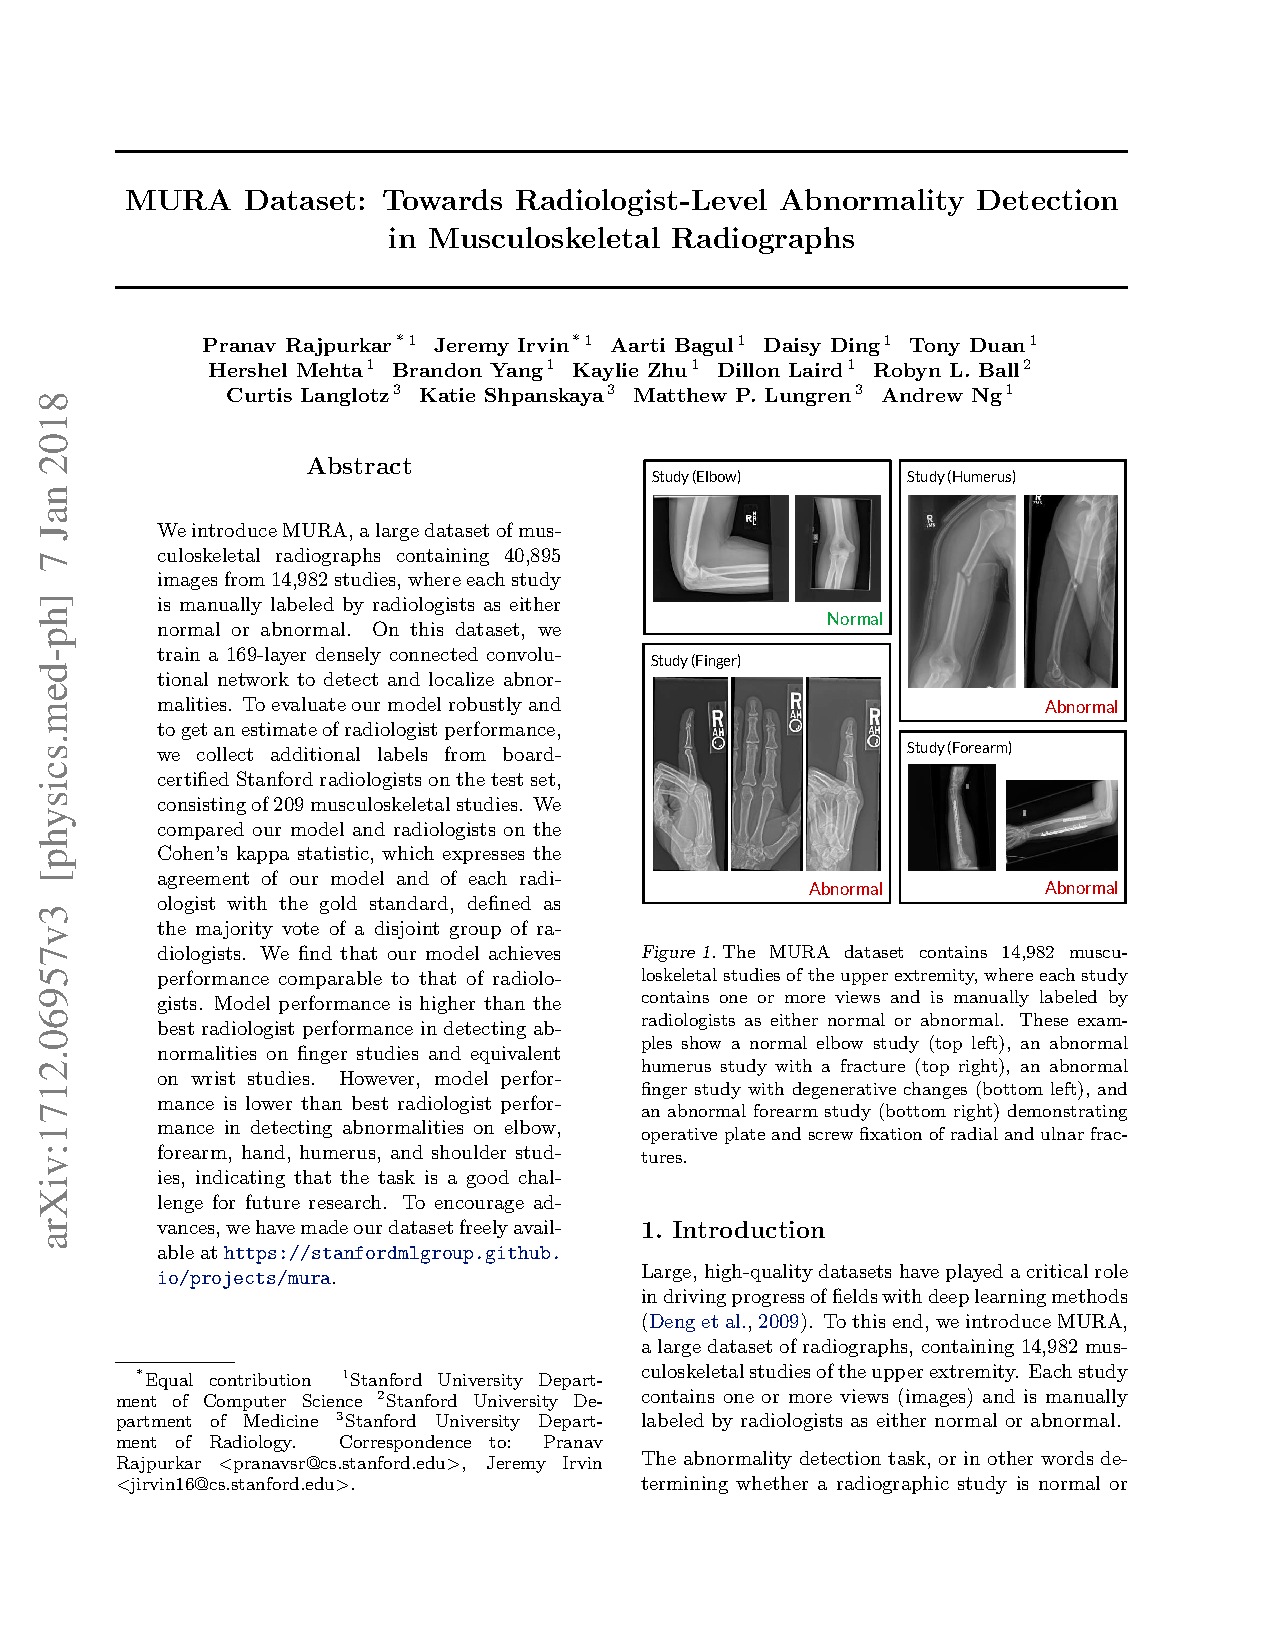
\includegraphics[
                    page=1,
                    width=\textwidth,
                    angle=0,
                    left
                ]{media/mura.pdf}
        \end{minipage}%
        \begin{minipage}{.49\textwidth}%
                \noindent
                \includegraphics[
                    page=2,
                    width=\textwidth,
                    angle=0,
                    right
                ]{media/mura.pdf}
        \end{minipage}%
    }
    \caption{Thumbnail of article by Rajpurkar et al. \autocite{MURA2017}}\label{fig:mura-image}
\end{figure}

MURA is one of the first large radiographic datasets focused exclusively on musculoskeletal imagery, as well as the name of a study conducted alongside said data by the Stanford Center for AI in Medical Imaging \autocite{MURA2017}. The MURA study marks a distinct landmark in the field of AI-assisted fracture classification, because it was the first to apply a deep-learning model on a large (40,561 radiographs), publicly available dataset. As a result, an examination of MURA allows us to contextualise our study in important ways: first, the success of MURA establishes the \emph{possibility} of using deep learning to robustly analyse radiography. Rajpurkar et al.~demonstrates near-radiologist levels of performance, validating the feasibility of our project in general. Secondly, the fact that the MURA model takes multi-view input imagery will help inform our own architectural design for processing both lateral and antero-posterior data. Finally, the limitations of MURA being a pure anomaly-detection system allows us to understand the need for a model which goes beyond binary classification, i.e.~what our project is trying to accomplish. 

To begin, it will be useful to look at MURA's architecture The MURA model is a 169-layer convolutional neural network which takes one or more views as input\footnote{Different views are radiographs of the same subject taken at different standard perspectives.}, and delivers a \emph{probability of anomaly}. The final probability is the arithmetic mean of output probabilities from every view \autocite{MURA2017}. Every type of radiograph may have multiple standard views, and the model architect has a choice of either training a model on a single view, or combining information from views in some ensemble stage. For anomaly detection, MURA chose a fairly conservative approach of assessing a separate probability of anomaly for each view, and then finding their average. This approach will be similar to the one that our project must take: which is to look at both the lateral and anteroposterior view of the tibia.

Another aspect of MURA that is worth examining, is their evaluation process. The model was accessed in two different ways: first, the model's precision versus recall plotted out in a Receiver Operating Characteristic (ROC) plot, and then the Area-Under-Curve of the ROC (AUROC) was quantified.  
\label{AUROC}
The AUROC is a common metric to assess diagnostic ability since it serves to quantify the precision-recall curve of the model. The MURA model had an AUROC of $0.929$. 
Second, a panel of three radiologists were assembled to evaluate a set of radiographs, and their performance was compared against the model. This kind of competitive evaluation allowed the study to compare the model performance against human clinicians, yielding an informative baseline for the AUROC.
With this information, we can contextualise the earlier AUROC value of $0.929$, and see that the model performs slightly worse than humans.

The use of AUROC as an evaluative metric, as well as competitive evaluation with human clinicians, present an advancement in model evaluation compared with the two earlier studies. However, in practice any AI model in radiography will not aim to replace human radiologists entirely, but serve as an additional tool which augments a human clinician's own diagnostic ability. Thus, the MURA study's evaluation is not representative of what real-world deployment would look like. This is why we must turn to Lindsey et al's \emph{Deep neural network improves fracture detection by clinicians}, for a more holistic example of model evaluation.

\section{Lindsey et al: Refinements to Model Evaluation}

\begin{figure}[H]
    \centering
    \fbox{%
        \begin{minipage}{.49\textwidth}%
                \noindent
                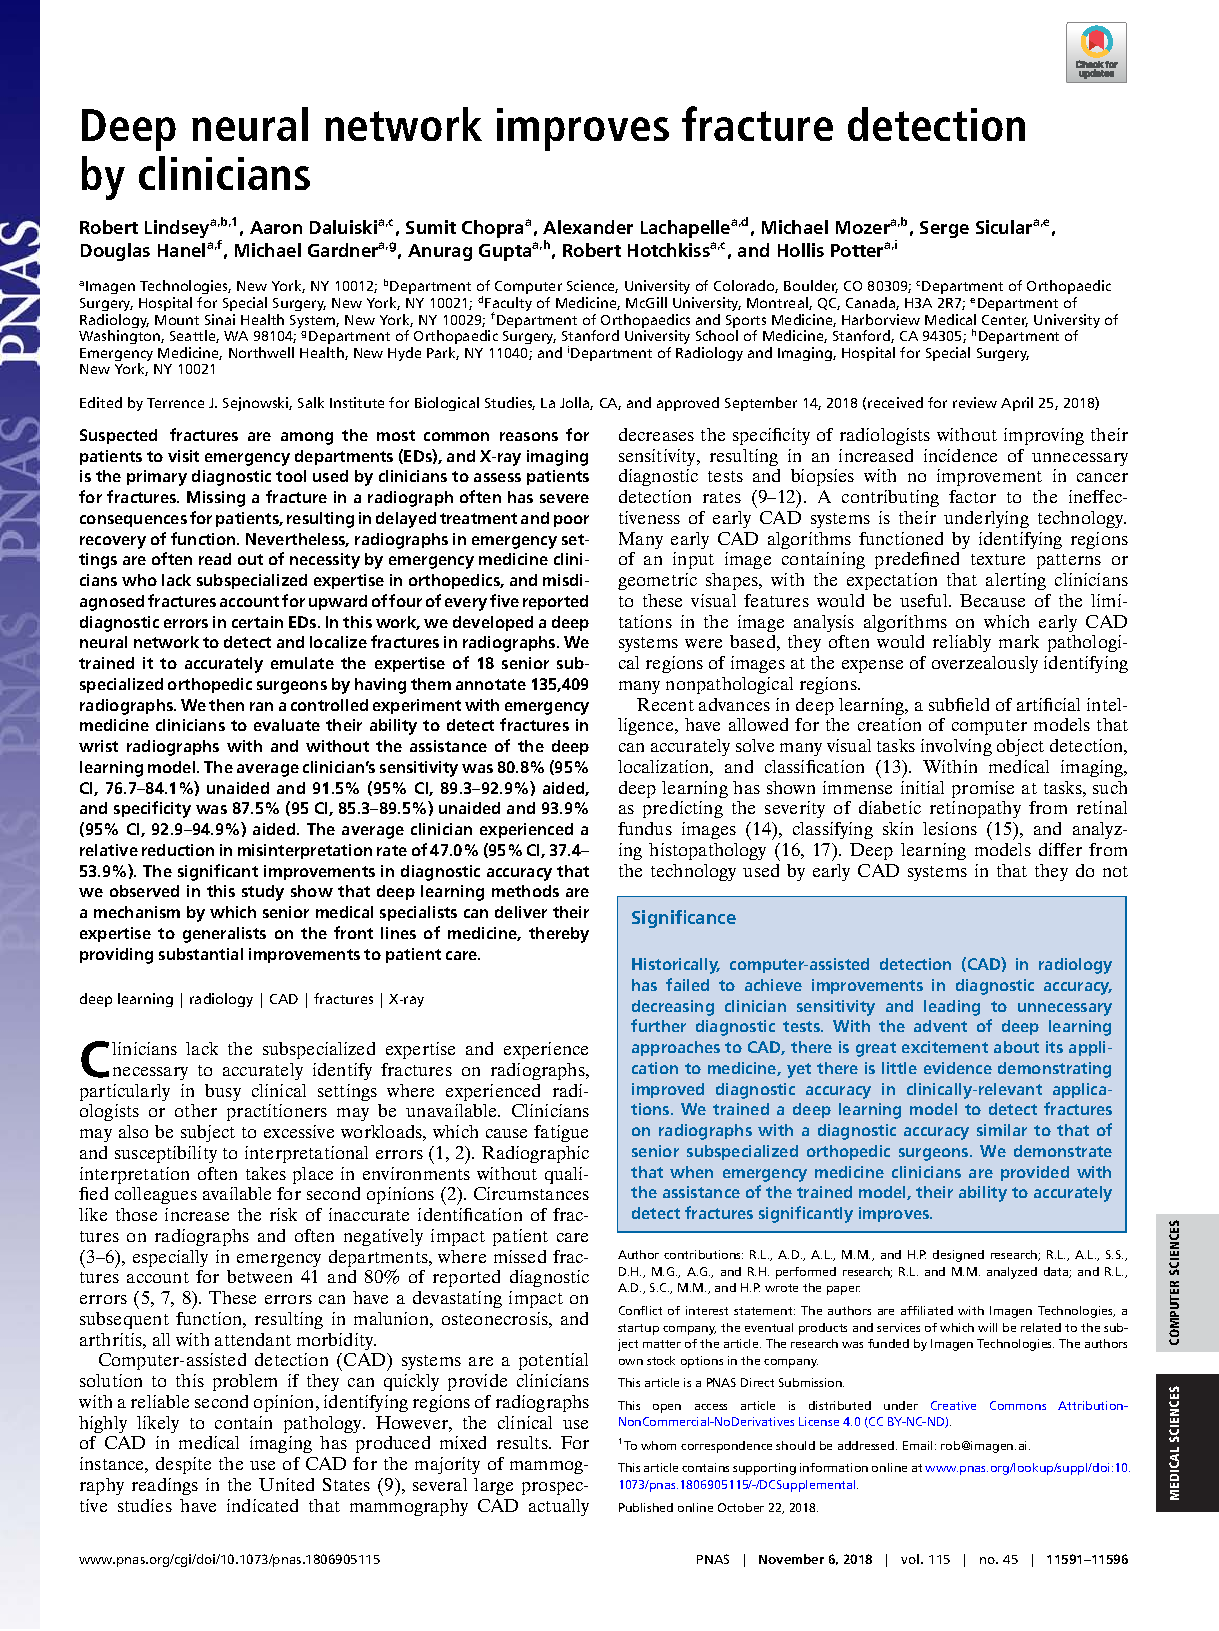
\includegraphics[
                    page=1,
                    width=\textwidth,
                    angle=0,
                    left
                ]{media/lindsey-et-al.pdf}
        \end{minipage}%
        \begin{minipage}{.49\textwidth}%
                \noindent
                \includegraphics[
                    page=2,
                    width=\textwidth,
                    angle=0,
                    right
                ]{media/lindsey-et-al.pdf}
        \end{minipage}%
    }
    \caption{Thumbnail of article by Lindsey et al. \autocite{Lindsey2018}}
    \label{fig:lindsey-image}
\end{figure}

In this study, a deep convolutional neural network is trained on a dataset of 31,490 wrist radiographs \autocite{Lindsey2018}. Like MURA, the study presents an AI-based fracture detection model, outputting both labels as well as a location heatmap. We include this study in the background research, for it's more holistic approach to evaluation, which simulates a real-world use-case. \textcquote{Lindsey2018}{Radiographic interpretation often takes place in environments without qualified colleagues available for second opinions}, the paper acknowledges, before proposing a model which aims to serve a possible \enquote*{second opinion.} After an initial evaluation which demonstrated an AUROC of $0.967$ on certain datasets\footnote{For model testing, the study utilised two distinct categories of radiographs divided into \enquote*{Test Set 1} and \enquote*{Test Set 2} (a slight improvement over MURA), with the former containing a collection of singleton wrist radiographs, and the latter of wrist radiographs with anterio-posterior and lateral views.}, Lindsey et al.~proceeds to conduct a second experiment, where a group of clinicians were shown radiographs from the same test set, and tasked to evaluate the radiograph both with and without the model's assistance:

\pagebreak
\blockcquote{Lindsey2018}{
    For each radiograph shown, the clinicians were asked whether or not
    a fracture was present. After a clinician made a response, the model's
    semantic segmentation prediction [i.e.~heatmap] was shown overlaid on the radiograph;
    the model's clinical determination was shown as text, and the clinician was asked the same question again.
}

\noindent
This experiment simulates the workflow of a clinician when using a fracture-detection model as a part of a CAD workflow. By doing so, we evaluate the effectiveness of the model as an useful tool within a broader clinical practice. The study found that the \textcquote{Lindsey2018}{\ldots\ sensitivity and specificity of the emergency medicine MDs were significantly improved with the assistance of the deep learning model.}

The key advantage of Lindsey et al's paper lies in its evaluative design, which our own project must take inspiration from. It may be impractical to setup a similar trial involving radiologists or clinical professionals,\footnote{Such an addition to this project is, however, within the realm of possibility, in collaboration with the medical faculty at METRC.} but one feature that we do aim to replicate is the output of a heatmap which highlights the location of features that the model detects. For the Lindsey et al.~and the MURA study, these heatmaps highlighted fracture-sights, whereas for our project they will highlight the sites of callus formation and bridging. By having this as a output, we will make the model's behaviour much more interpretable, and allow for integration into real clinical workflows.

\section{Kim \& MacKinnon: Cross-Domain Transfer Learning}

\begin{figure}[H]
    \centering
    \fbox{%
        \begin{minipage}{.49\textwidth}%
                \noindent
                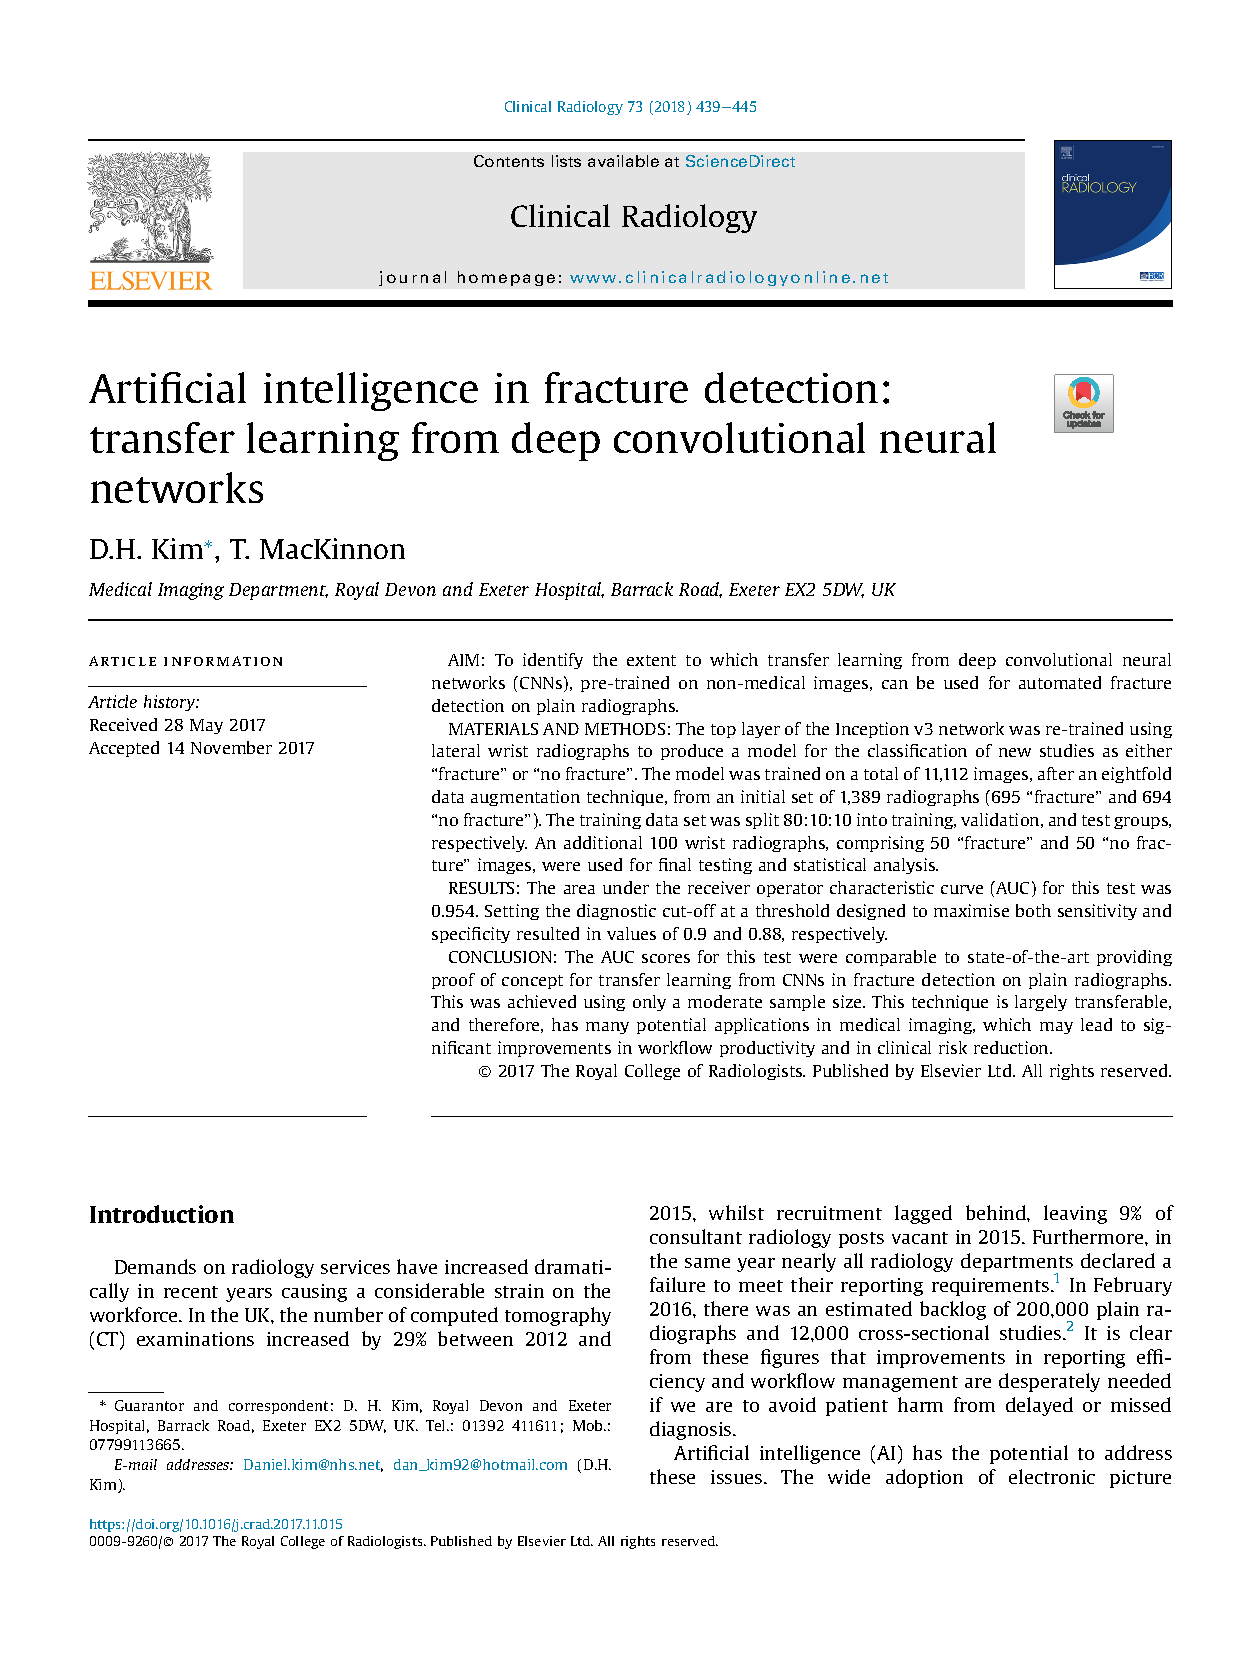
\includegraphics[
                    page=1,
                    width=\textwidth,
                    angle=0,
                    left
                ]{media/kim-and-mackinnon.pdf}
        \end{minipage}%
        \begin{minipage}{.49\textwidth}%
                \noindent
                \includegraphics[
                    page=2,
                    width=\textwidth,
                    angle=0,
                    right
                ]{media/kim-and-mackinnon.pdf}
        \end{minipage}%
    }
    \caption{Thumbnail of article by Kim and MacKinnon. \autocite{Kim2018}}\label{fig:kim2018-image}
\end{figure}  

Studies \autocites{MURA2017}{Lindsey2018} both rely on large, labelled radiographic datasets. While such datasets exist for fracture \emph{detection} and fracture 
\emph{classification}, the classification of fracture healing by their RUST scores is without precedence in literature, and to our knowledge there are no openly available datasets with the aforementioned labels. For our project, we will be using radiographic data internally collected by the \href{https://www.metrc.org/}{Major Extremity Trauma Research Consortium} (METRC), a research unit at the Johns Hopkins Bloomberg School of Public Health. Although this dataset has the RUST-scores we require, the number of radiographs we have access to is limited. Hence our approach is to utilise \emph{transfer learning}, a process where the model is first trained on a larger, general-purpose dataset, before being fine-tuned on the study data. Thus, we turn to Kim and MacKinnon's \emph{Artificial intelligence in fracture detection} for their innovative use of transfer learning.~\autocite{Kim2018}

In Kim and MacKinnon's study, a dataset of 1,389 radiographs was available for a binary classification task (i.e.~labels were \enquote{fracture} or \enquote{no fracture}). Instead of training a model \emph{ab initio}, a CNN trained on a general purpose, non-radiographic dataset was re-applied on the radiography data. The authors used the Inception v3 network, an object-detection and image classification network  \autocite{Szegedy2016} with the topmost layer fine-tuned on the radiographic data. \autocite{Kim2018}. By using a pre-existing model and data augmentation\footnote{The authors of \autocite{Kim2018} ultimately generated 11,112 augmented samples from their initial set of 1,389 radiographs.}, Kim and MacKinnon were able to achieve an  AUROC of $0.954$, a value that is within the same standard deviation of \autocites{MURA2017}{Lindsey2018}, studies which both had much larger datasets for their models.

Our inclusion of Kim and MacKinnon's study serves as an important validation for the aims of our project. The METRC dataset will consist of around two to three thousand radiographs sourced from a handful of METRC studies. If Kim and MacKinnon's model is already able to achieve a robust performance with only 1,389 samples, than it is quite possible for our own project to achieve it's aims. The theoretical reasoning behind why transfer learning can achieve high levels of model performance is because the first layers of a CNN are primarily responsible for high-level feature extraction, e.g.~edge detection, pattern recognition, with only the latter layers responsible for task-specific classification \autocite{Kim2018}. This does, however open up a further avenue of inquiry. Would model performance improve further, if the base model that the transfer learning is conducted from, was itself originally trained on a domain-specific dataset, like the MURA data from \autocite{MURA2017}? Our project will explore this possibility, through it's own application of transfer learning to the prediction of radiographic union with RUST scores.

% I should look at three different papers in depth.

% This one also looks at AT/L views
% https://pubmed.ncbi.nlm.nih.gov/30348771/

% MURA: Large dataset
% https://arxiv.org/pdf/1712.06957.pdf

% Transfer Learning
%  https://www.clinicalradiologyonline.net/article/S0009-9260(17)30535-4/fulltext


% Methedology: 2,000 words

\chapter{Methodology}

The primary objective of our study is to develop an AI model using the technique of transfer-learning, to automatically predict RUST scores from an input radiograph. In this chapter, we will first discuss our experiment design, contextualising the choices we make in our methodology and evaluation. Next, we will briefly summarise the datasets used in the study, before proceeding to the main methodology (protocols) itself. Afterwards, the evaluation and endpoints will be presented, as well as a discussion on patient privacy and ethical considerations.

\section{Model Design}

Transfer learning is a technique which uses a model trained upon a larger dataset first, before being applied to a smaller, task-specific dataset. Assuming our task-specific dataset (in our case, the RUST data from METRC) is fixed, the performance of our transfer-learning model is determined by the following factors:

\begin{enumerate}
    \item The architecture of the original model.
    \item The initial, large dataset that the original model is trained on.
\end{enumerate}

\noindent
Hence, in the context of our study design, we must first choose (or create) a model architecture, and select an initial large dataset to train our model on. Only then are we able to apply the transfer learning procedure (e.g. freeze model weights, add new classifier, fine tuning, etc) upon our task-specific dataset.

\subsection{Model Architecture Choices}

The first decision that we must make in our experiment design is the choice of model architecture.
According to a literature survey by Litjens, Kooi, Bejnordi et al., convolutional neural networks (CNNs) are the most common deep learning architecture deployed for medical image analysis, vastly outnumbering alternative methods such as Stacked Autoencoders (SAE), or Recurrent Neural Networks (RNNs) \autocite[77]{cnn-most-common}.
This is expected, as CNNs exhibit strong performance with image classification tasks, and as our project is an image classification task (albeit with radiographs), we will be using a CNN.

The choice now remains to either design our own CNN from scratch, or use an existing CNN architecture.
Although designing a CNN \emph{ab initio} allows the possibility of further experimentation and potentially finer-grained control, such a \emph{de novo} model is difficult to assess holistically: there would be no prior work in literature to serve as a basis for comparison.
In contrast, if we use a well-documented, existing CNN as our transfer-learning foundation, we may compare the performance of our implementation against other instances of the same model architecture used for transfer-learning in different domains.
% The commensurability of a standard model for comparison is important: in a 2022 review of transfer learning techniques in medical image analysis, Kora, Ooi, Faust et al. found that only 13\% of prior studies compared their results with other models \autocite[94]{kora2022}. 

Thus, we will be using the InceptionV3 model, a convolutional neural network developed by Szegedy, Vanhoucke, Ioffe, et al. from Google \autocite{inceptionv3}. Our choice of InceptionV3 is based upon a 2022 literature review of transfer-learning models for the domain of medical image analysis. According to Kora, Ooi, Faust et al., CNNs with a broad (as opposed to deep) network topology perform well in transfer-learning tasks \autocite{kora2022}, with models like InceptionV3 outperforming more parameterized models like AlexNet \autocite{alexnet}. Indeed out of the 54 studies included in the review, Inception-style models both the most common (14 out of 54) and among the highest-performing. \autocite{kora2022}

\subsection{\enquote*{Top-Classifier} Choices}

\emph{This subsection is unavailable in this version of the document.}

\subsection{Model Optimizer Choices}

Finally, the last architectural decision we must make in our model design, is the choice of an optimizer. We have two possible approaches: we may either select an optimizer from \emph{a priori} principles, or consider the selection of an optimizer to be a hyperparameter, and benchmark a variety of optimizers with our model on the data-set. Because we are already evaluating two variants of InceptionV3, the additional task of iterating through different optimizers will be infeasible given the time and compute constraints of the project.

Hence, our choice of an optimizer is determined by a review of available benchmarks and literature. The study and benchmarking of deep learning optimizers is a fairly recent field, initiated by the development of robust, reproducible benchmarks. Projects like Schneider, Balles, et Hennig's \emph{DeepOBS: A Deep Learning Optimizer Benchmark Suite} allowed researchers to evaluate optimizers against an assay of realistic optimization problems, simulating common deep learning tasks and neural network architectures. \autocite{deepobs} The availability of reproducible benchmarks allowed the first large-scale empirical experiments to be conducted on optimizer performance, culminating in Schmidt, Schneider, et Hennig's 2021 paper in optimizer benchmarking. \autocite{crowdedvalley} In an evaluation of 15 popular optimizers\footnote{AMSBound, AMSGrad, AdaBelief, AdaBound, AdaDelta, Adam, LookaheadMomentum, LookaheadRAdam, Momentum, NAG, NAdam, RAdam, RMSProp, and SGD, respectively. The full list of results are available in their supplementary appendix.} across a total of more than 50,000 epochs of training, significant data on optimizer performance was gathered.

Of the eight optimization problem assays in the benchmark suite, our task of radiographic image classification is bears closest resemblance to the CIFAR-10 benchmark: a CNN-based image classification task. According to the latest results available on the paper's website\footnote{\url{https://deepobs.github.io/leaderboardP4.html}}, the ADAM optimizer has a slight accuracy improvement over Momentum and SDG. However, the differences are so small that the author mentions: \blockcquote[2]{crowdedvalley}{
    \ldots\ a practitioner with a new deep learning task can expect to do about equally well by taking almost \emph{any method} from our benchmark and tuning it, as they would by investing the same computational resources into running a set of optimizers with their default settings and picking the winner.
}

\noindent
Therefore, we will select the ADAM optimizer, and spend time on fine-tuning the model and hyperparameter choices, instead of devoting further resources to selecting an optimizer.

\subsection{Pre-Training Dataset Choices}

Now that we decided our model architecture, the next step is to select the initial, or pre-training dataset, that is used to train our model.

\subsubsection{ImageNet Dataset}
Originally, InceptionV3 was trained on the ImageNet dataset: a general-purpose collection of more than 14 million everyday images. \autocite{imagenet} The overwhelming size of the ImageNet dataset serves as a robust foundation for the InceptionV3 model, which exhibits strong performance in classification tasks upon it. However, the statistical characteristics of data in ImageNet is quite different from data in a typical radiography dataset. Hence, it remains a valid research question to ask whether a InceptionV3 model trained on a smaller, but more domain-specific dataset will exhibit better performance when applied to our transfer-learning task.

\subsubsection{RadImageNet Dataset}
Thus, we will also investigate RadImageNet, a collection of 5 million medical images composing of radiographic (CT), MRI, and ultrasound images. \autocite{radimagenet} As an open radiologic dataset developed specifically for transfer learning applications, a base model trained on RadImageNet may exhibit better performance on our radiography data, as the original network is trained upon images in a similar domain. However, the advantages of a similar domain is moderated by the corresponding smaller dataset size (5 million versus ImageNet's 14 million).

Therefore, in this project we will evaluate the use of a InceptionV3 model trained both on the ImageNet dataset, as well as the RadImageNet dataset as the base model for transfer learning. By comparing the performance of both models, we will be able to select the best-performing one for further development and refinement. Additionally, the additional data point afforded by a second model allows greater context for our evaluation: according to Kora et al., only 13\% of transfer-learning studies benchmarked their model performance against a second model. \autocite[94]{kora2022} By choosing to evaluate two models from the very start of our project's design, we get to avoid this scientific blind-spot: and hopefully achieve a better result overall.

\section{Data Egress and Preprocessing}

Now that we have defined the design of our experiment, we must define the pre-processing and data egress requirements.
Our study data consists of anteroposterior and lateral view radiographs, as well as their corresponding RUST scores. This data is provided in a collaboration with METRC, Johns Hopkins University, through their archive of past and on-going studies. \autocites{RetroDEFECT2022}{OUTLET2021}{PAIN2017}{PACS2022} The data is held within REDCap: an electronic data and clinical trials database. \autocite{redcap} Because the data is held across multiple clinical trials and within multiple instruments, egressing data out of REDCap and pre-processing it into a useable form is a non-trivial software engineering task.

\begin{table}[H]
    \centering
    \begin{tabularx}{\textwidth}{@{}lXr@{}}
    \toprule
    \textbf{Dataset}     & \textbf{Name} & \textbf{Samples} \\ \midrule
    \autocite{RetroDEFECT2022} \textsc{RetroDEFECT} & \emph{Retrospective Study of the Treatment of Long Bone Defects}    & $741$             \\
    \autocite{OUTLET2021} \textsc{Outlet}      & \emph{Outcomes Following Severe Distal Tibia, Ankle and/or Foot Trauma}     & $707$             \\
    \autocite{PAIN2017} \textsc{Pain}        & \emph{Pain Management \& Long Term Outcomes Following High Energy Orthopedic Trauma}      & $370$             \\
    \autocite{PACS2022} \textsc{Pacs}        & \emph{Predicting Acute Compartment Syndrome using Optimized Clinical Assessment}    & $195$             \\ \midrule
    Sum         &      & $2,013$            \\ \bottomrule
    \end{tabularx}%
    \caption{Sources of Radiographic Data with RUST labels in REDCap}\label{tab:datasets}
\end{table}

\subsection{Validate Radiography Data with Branch-Parser}

The first challenge that we face in the data egress process, is finding RUST-radiography pairings that are valid for inclusion in our dataset. A small subset of radiographs do not possess valid RUST scores: either because they were uninterpretable due to hardware occlusion (e.g. presence of a titanium orthopaedic fixture), or because the radiograph was not taken for the purpose of assessing fracture healing. In order to validate the radiography data, a Python package called redcap-branch-parser was developed to parse the conditional logic contained within REDCap patient records. \autocite{redcap-branch-parser} The development of this package took up a non-trivial amount of early project work.

Once valid RUST-radiograph pairs were identified, the study data was egressed out of REDCap using a set of ad-hoc Jupyter Notebooks and the PyCap API package. \autocite{pycap}

\subsection{Automated de-skewing with ImageMagick}
Following the egress of radiography data, the radiography image files were automatically de-skewed using ImageMagic. At this point, data-preprocessing is complete, as data augmentation will be performed dynamically via layers within Keras.

\section{Data Augmentation Strategy}

Because we have a small dataset, a robust data augmentation strategy is needed to combat overfitting. In order to develop our data augmentation strategy, we followed suggestions from Bejani et Ghatee's \emph{systematic review on overfitting control in shallow and deep neural networks} \autocite{overfitting-prevention}. We may categorise data augmentation strategies to three broad families of methods: \autocite{augmentation-strategies}

\begin{enumerate}
    \item \textbf{Geometric Methods:} rotation, cropping, flipping.
    \item \textbf{Photometric Methods:} noise, color-shifting, edge modification.
    \item \textbf{\enquote*{Complex} Methods:} generating artificial data using GANs, style transfer.
\end{enumerate}

\noindent
Of the three, \enquote*{complex} data augmentation methods such as generating artificial data points is inappropriate for our use case, as it will compromise the evidence-based labelling of our dataset. Hence, we may recourse to either geometric methods, or photometric methods. Originally, our intuition was that photometric data augmentation methods would be of limited applicability to radiographs, which are entirely greyscale. Upon further investigation, it turns out that when evaluated individually, the most effective data augmentation strategy is cropping, followed by rotation. \autocite{benchmark}

Hence, in order to avoid potentially compromising our small dataset with too much noise, our data augmentation strategy will be restricted to geometric methods such as rotation, cropping, and flipping.

\clearpage

\section{Protocols}

Now that we have finished discussing the model design, data egress, and augmentation, it is time to define the study protocols. The experimental portion of this study will consist of three protocols:

\begin{enumerate}
    \item Protocol   I: A \enquote*{naive} CNN without transfer-learning, for use as a baseline.
    \item Protocol  II: Transfer-learning w/ InceptionV3 trained on ImageNet.
    \item Protocol III: Transfer-learning w/ InceptionV3 trained on RadImageNet.
\end{enumerate}

\noindent
All protocols will utilise the same data augmentation pipeline.

\begin{figure}[H]
    \centering
    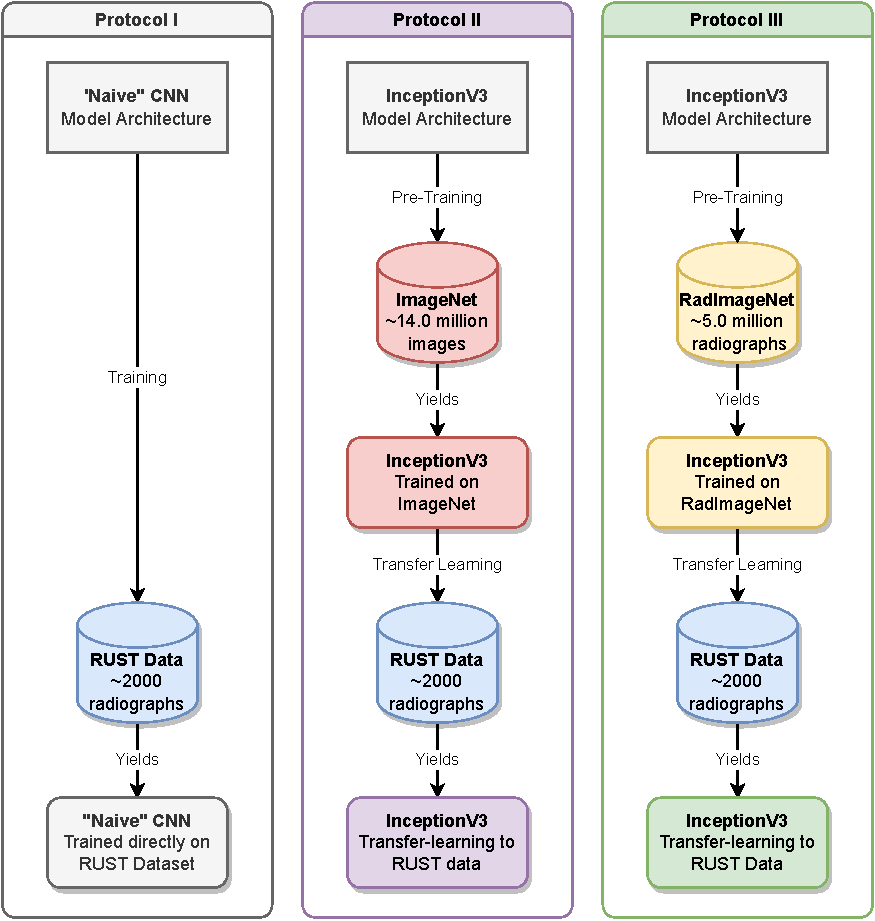
\includegraphics[
        page=1,
        width=\textwidth,
        angle=0,
        right
    ]{media/protocol-diagram.pdf}
    \caption{Overview illustrating the three model development protocols.}
    \label{fig:protocols}
\end{figure}

\subsection{Protocol I: \enquote*{Naive} CNN Baseline}

In protocol I, we will develop a \enquote*{naive} CNN without the use of transfer learning, that is trained directly on the RUST dataset. This model will serve as a performance baseline to benchmark our transfer-learning models against.

\subsubsection{\enquote*{Naive} CNN Architecture}

\emph{This subsection is unavailable in this version of the document.}

\subsection{Protocol II: InceptionV3 with ImageNet}

In protocol II, we will use InceptionV3 trained on the ImageNet dataset as a base model for transfer-learning.

\noindent
\emph{This is an outline. More information will be added later.}

\begin{enumerate}
    \item Instantiate base model with pre-trained weights.
    \item Freeze weights in base model. Remove output (classifier) from base model.
    \item Create a new classifier on top of base model.
    \item Create input augmentation pipeline using keras layers.
    \item Normalise RUST dataset towards mean and standard deviation of ImageNet dataset
    \item Compile model with optimizer settings.
    \item Train classifier (i.e. top layer).
    \item Unfreeze weights in base model.
    \item Perform one additional round of training with a very small learning rate, for fine-tuning.
    \item Evaluate model performance.
\end{enumerate}

\subsection{Protocol III: InceptionV3 with RadImageNet}

In protocol II, we will use InceptionV3 trained on the RadImageNet dataset as a base model for transfer-learning.

\noindent
\emph{This is an outline. More information will be added later.}

\begin{enumerate}
    \item Instantiate base model with pre-trained weights.
    \item Freeze weights in base model. Remove output (classifier) from base model.
    \item Create a new classifier on top of base model.
    \item Create input augmentation pipeline using keras layers.
    \item Normalise RUST dataset towards mean and standard deviation of ImageNet dataset
    \item Compile model with optimizer settings.
    \item Train classifier (i.e. top layer).
    \item Unfreeze weights in base model.
    \item Perform one additional round of training with a very small learning rate, for fine-tuning.
    \item Evaluate model performance.
\end{enumerate}

\section{Hyperparameter and Learning Rate Tuning}

The hyperparameter and learning rate tuning is only applicable to \emph{either} Protocol II or Protocol III, depending on which was the better-performing one.

\subsection{Hyperparameter Tuning Regime I}

\emph{This subsection is unavailable in this version of the document.}

\subsection{Hyperparameter Tuning Regime II}

\emph{This subsection is unavailable in this version of the document.}

\subsection{Learning Rate Schedule}

\emph{This subsection is unavailable in this version of the document.}

\section{Evaluation and Endpoints}

Assuming an available dataset of \(\approx2,000\) samples (after removing invalid entries), we will be setting aside \(15\%\) of the initial data (\(\approx300\) samples) for the testing dataset.

\subsection{AUROC}

Model performance will be assessed via AUROC, the Area-Under-Curve of the Receiver Operating Characteristic (ROC) graph. This is the area underneath the precision-versus-recall plot of the model, and is a common metric used to assess diagnostic accuracy.

\subsection{K-Fold Cross-Validation}

Due to the small size of our dataset, we will be using K-Fold Cross validation as a technique to get a more accurate assessment of our model performance. Instead of setting aside a hold-out validation set of \(15\%\) (i.e. \(\approx300\) samples out of the initial \(\approx 2,000\)), we will be running \(k=5\) folds on the \(1,700\) sample data. This yields \(\approx 340\) samples per validation fold, which approximates the usual \(\approx300\) samples of a regular hold-out validation set.

\subsection{Endpoints}
First, prior to assessing model performance, we want to determine:

\begin{enumerate}
    \item \emph{Does InceptionV3 trained on the domain-specific RadImageNet dataset perform better as a transfer-learning base on our RUST dataset?}
\end{enumerate}

\noindent
Protocol I and Protocol II will allow us to answer that research question. Once we have found the best-performing variant of InceptionV3, we will then begin the process of optimising model performance as measured through AUROC. For performance, we aim to achieve the following endpoints:

\begin{enumerate}
    \item Endpoint 1: AUROC > 0.50
    \item Endpoint 2: AUROC > \enquote*{Naive} CNN
    \item Endpoint 3: AUROC > 0.75
\end{enumerate}

\noindent
Initially, we aim to achieve an AUROC that is greater than chance, which is the minimal backstop to model performance. Failure to reach this endpoint will indicate severe flaws with our study design, such as our dataset being too small for even transfer-learning to be applicable. Following that, we want to exceed the performance of our \enquote*{naive} CNN. Finally, we wish to validate the concept of using AI to infer RUST scores from radiographs, by achieving an AUROC that is greater than 0.75.

\section{Feasibility and Proof of Concept}

Right now, a significant and on-going challenge is completing the initial data egress and pre-processing. As the study dataset is still not assembled and ready to use yet, initial feasibility and proof of concept experiments can be conducted on a readily available dataset from a similar domain, such as the MURA musculoskeletal radiography data from Stanford. By beginning with an artificially constrained subset of images and labels from MURA, we may validate our transfer learning protocol and gather some preliminary information.

\subsection{Experiments with the MURA Dataset}

\emph{This subsection is unavailable in this version of the document.}

\subsection{Preliminary Results}

\emph{This subsection is unavailable in this version of the document.}

\section{Ethical Considerations}

Any research project or study that involves human subjects will necessitate ethical consideration. This section is only a brief discussion of ethical risks and mitigations. The aim of this project is to validate transfer learning as a technique to infer RUST scores from a small dataset of radiographs. Although we aim to achieve robust performance in order to demonstrate the feasibility of this technique as an avenue for further research, at no time do we imply to develop a \emph{diagnostic} tool for clinical use. The overarching spirit of the study is to explore interdisciplinary applications of AI in medical imaging, in hopes of reducing clinical caseload for medical practitioners, leading to better standards of care for all patients overall. This overarching goal is a positive one, which aims to improve health and healthcare for all.

\subsection{Human Radiographic Data}

This study works with radiographs collected from human subjects, that were a part of past or on-going METRC studies in high-energy trauma. This data is fully anonymised, and does not contain any personally identifiable information. 

\subsection{Human Subject Research, and HIPAA Compliance}

As a part of Johns Hopkins Bloomberg School of Public Health's IRB requirements, all researchers working with human data, even anonymised data, must complete a Human Subject Research certification, and a Information Privacy Security certification.  

\chapter{Implementation and Analysis}\label{implementation}

In this chapter, we will present the implementation of the study methodology. Recall that the methodology has three components. We will begin with the establishment of an initial baseline, by creating and training a classical \enquote*{shallow} convolutional neural network based upon LeCun et al.'s 1998 LeNet model. \autocite{lenet1998} This classical CNN baseline will serve as the minimal performance standard that our model will aim to surpass. Next, utilising the InceptionV3 architecture which will serve as our transfer-learning base model, we will train an end-to-end (i.e.\ without transfer learning) model on our radiography dataset. This will serve as an additional baseline that will allow us to validate the transfer-learning \emph{technique} against regular end-to-end training.

Following the establishment of these two baselines, we will proceed to begin an initial evaluation of two different transfer-learning base models. We will compare the performance of InceptionV3 trained with ImageNet weights \autocite{imagenet}, against InceptionV3 trained with RadImageNet \autocite{radimagenet} weights. This initial evaluation will help us explore whether a base model trained on the smaller, but domain-specific RadImageNet dataset will have any advantages over the larger, but general ImageNet dataset. We will select the better performing base model out of the two options, and proceed to optimize the model's hyperparameters.

Our model's hyperparameter search procedure consists of two steps, which we term hyperparameter search Regime I and hyperparameter search Regime II. As per our methodology, in Regime I we find the optimal batch size and dropout rate for our model. This is done using a stochastic search process where the hyperparameter space of the model is randomly sampled for \(t\) trials, where each trial consists of a k-fold cross-validation of the model with the selected hyperparameters. Once the optimal combination of batch size and dropout rate are found, we will set these hyperparameters as constant and proceed to the second hyperparameter search regime. In Regime II we find the optimal learning rate and epsilon value \(\epsilon\) for the Adam optimizer, by conducting a grid search over a selection of possible values.

\section{K-Fold Evaluation}

Before we begin, we must first implement our k-fold cross-validation routine. Since model performance is sensitive to the network's random weight initialisation\footnote{This is particularly true on small datasets with unbalanced classes like ours.} \autocite{Narkhede2022}, our methodology requires k-fold cross-validation to be conducted on every experiment (i.e.\ model run). My implementation of the k-fold cross-validation process consists of two parts: a function which will divide the dataset into \(k\) folds, as well as a function that runs the k-fold cross-validation on the given model. The the \mintinline{python}{k_fold_dataset()} function is given as follows:\footnote{The code listings provided in this document \emph{are for illustration only}. The actual implementation is generally longer, and contains docstrings, debugging instrumentation, file I/O logic, as well as additional function arguments. Every listing will have a link to it's corresponding implementation in the git repository.}

\begin{listing}[H]
        \begin{minted}[
            baselinestretch=1.0,
            frame=lines,
            mathescape,
            autogobble,
            fontsize=\footnotesize,
            style=default,
            breaklines,
            breakbytoken
        ]{python}
        def k_fold_dataset(ds: tf.data.Dataset, k: int = 10) -> list[tuple[tf.data.Dataset, tf.data.Dataset]]:
            # First shard the given dataset into k individual folds.
            list_of_folds: list[tf.data.Dataset] = []
            for i in range(k):
                fold: tf.data.Dataset = ds.shard(num_shards=k, index=i)
                list_of_folds.append(fold)
        
            # Next, generate a list of train and validation dataset tuples
            list_of_ds_pairs: list[tuple[tf.data.Dataset, tf.data.Dataset]] = []
            for i, holdout_fold in enumerate(list_of_folds):
                ds_valid: tf.data.Dataset = holdout_fold
        
                # Select every fold except holdout_fold as the training folds
                training_folds: list[tf.data.Dataset] = list_of_folds[:i] + list_of_folds[i+1:]

                # ds_train size is $\frac{k-1}{k}$ of the original dataset
                ds_train: tf.data.Dataset = training_folds[0]
                for fold in training_folds[1:]:
                    ds_train = ds_train.concatenate(fold)
        
                ds_pair: tuple[tf.data.Dataset, tf.data.Dataset] = (ds_train, ds_valid)
                list_of_ds_pairs.append(ds_pair)
            
            return list_of_ds_pairs
        \end{minted}
    \caption{Sharding dataset for K-Fold Cross Validation (\href{https://github.com/ShenZhouHong/radiography-ai-project/blob/cf8c9e9a1f07849787a98b2fc51df690354bf194/python/common/kfold.py}{Github})}\label{listing:sharding}
\end{listing}

\noindent
One thing of note, is that our \mintinline{python}{k_fold_dataset()} function conducts all dataset-related operations using the Tensorflow's high-performance \mintinline{python}{tf.data.Dataset} API. This allows support for pre-fetch, caching, and other low-level optimisations. This function serves as a dependency which is called by \mintinline{python}{cross_validate()}, which runs the actual K-fold cross validation experiments on the given model:

\begin{listing}[H]
        \begin{minted}[
            baselinestretch=1.0,
            frame=lines,
            mathescape,
            autogobble,
            fontsize=\footnotesize,
            style=default,
            breaklines,
            breakbytoken
        ]{python}
        def cross_validate(ModelClass: tf.keras.Model, ds: tf.data.Dataset, epochs: int = 50, batch_size: int = 128, k: int = 10) -> list[tf.keras.callbacks.History]:

            history_list: list[tf.keras.callbacks.History] = []
            train_valid_pairs: list[tf.data.Dataset] = k_fold_dataset(ds, k)
        
            for i, (ds_train, ds_valid) in enumerate(train_valid_pairs):
        
                tf.keras.backend.clear_session()
                model = ModelClass()
                model.compile(
                    optimizer=tf.keras.optimizers.Adam(),
                    loss=tf.keras.losses.BinaryCrossentropy(),
                    metrics=metrics
                )
                history = model.fit(
                    ds_train,
                    validation_data=ds_valid,
                    epochs=epochs,
                    batch_size=batch_size,
                )
                history_list.append(history.history)

            return history_list
        \end{minted}
    \caption{K-Fold Cross Validation Implementation}\label{listing:cross-validate}
\end{listing}

\noindent
The output of every k-fold cross-validation experiment will be a \enquote*{history list} containing \(k\) \mintinline{python}{tf.keras.callbacks.History} objects. This \mintinline{python}{History} object will contain training and validation metrics which will be used to calculate the average metric over \(k\) folds:

\begin{listing}[H]
    \begin{minted}[
        baselinestretch=1.0,
        frame=lines,
        mathescape,
        autogobble,
        fontsize=\footnotesize,
        style=default,
        breaklines,
        breakbytoken
    ]{python}
    def calculate_mean_metrics(kfold_metrics: list[dict[str, float]]) -> dict[str, list[float]]:
        # Initialise aggregate metrics with appropriate keys
        aggregate_metrics: dict[str, list[float]] = {}
        for fold in kfold_metrics:
            for metric in fold.keys():
                if metric not in aggregate_metrics:
                    aggregate_metrics[metric] = []

        # Calculate the average metric per epoch for every fold
        number_of_folds: int = len(kfold_metrics)
        for metric in aggregate_metrics.keys():
            number_of_epochs: int = len(kfold_metrics[0][metric])
            for epoch in range(number_of_epochs):
                # A list of every value for that given metric in this epoch across folds
                values_per_epoch: list[float] = [x[metric][epoch] for x in kfold_metrics]
                mean_per_epoch  : float = sum(values_per_epoch) / number_of_folds
                aggregate_metrics[metric].append(mean_per_epoch)

        return aggregate_metrics
    \end{minted}
\caption{Calculating Mean Metrics from K-Fold Data (\href{https://github.com/ShenZhouHong/radiography-ai-project/blob/52b2674f328c7595a32b7e4bcd2c6d4d4824e4ca/python/common/utilities.py}{Github})}\label{listing:calc-mean-metrics}
\end{listing}


\noindent
The above code now completes the prerequisites necessary for data gathering.

\section{Establishing a Baseline}

\subsection{Shallow Convolutional Neural Network}

\begin{listing}[H]
    \begin{minted}[
        baselinestretch=1.0,
        frame=lines,
        mathescape,
        autogobble,
        fontsize=\footnotesize,
        style=default,
        breaklines,
        breakbytoken
    ]{python}
    class LeNet1998(tf.keras.Model):
        def __init__(self, **kwargs):
            super().__init__(**kwargs)

            self.input_layer: tf.Tensor = layers.InputLayer(input_shape=(299, 299, 3))
            self.data_augmentation: tf.keras.Sequential = tf.keras.Sequential([
                layers.RandomFlip(seed=RNG_SEED),
            ])

            self.lenet1999: tf.keras.Model = tf.keras.Sequential([
                layers.Conv2D(6, kernel_size=5, strides=1,  activation='tanh', padding='same'),
                layers.AveragePooling2D(),
                layers.Conv2D(16, kernel_size=5, strides=1, activation='tanh', padding='valid'),
                layers.AveragePooling2D(),
            ])

            self.classifier: tf.keras.Sequential = tf.keras.Sequential([
                layers.Flatten(),
                layers.Dense(1024, activation='relu'),
                layers.Dense(18, activation='sigmoid')
            ])

            self.model: tf.keras.Sequential = tf.keras.Sequential([
                    self.input_layer,
                    self.data_augmentation,
                    self.lenet1999,
                    self.classifier
            ])

        def call(self, inputs):
            return self.model(inputs)
    \end{minted}
\caption{The LeNet 1998 Shallow CNN Model (\href{https://github.com/ShenZhouHong/radiography-ai-project/blob/cf8c9e9a1f07849787a98b2fc51df690354bf194/python/initial-evaluation/lenet1998.ipynb}{Github})}\label{listing:lenet1998}
\end{listing}

\begin{listing}[H]
    \begin{minted}[
        baselinestretch=1.0,
        frame=lines,
        mathescape,
        autogobble,
        fontsize=\footnotesize,
        style=default,
        breaklines,
        breakbytoken
    ]{python}
    class LeNet1998(tf.keras.Model):
        def __init__(self, **kwargs):
            super().__init__(**kwargs)

            self.input_layer: tf.Tensor = layers.InputLayer(input_shape=(299, 299, 3))
            self.data_augmentation: tf.keras.Sequential = tf.keras.Sequential([
                layers.RandomFlip(seed=RNG_SEED),
            ])

            self.lenet1999: tf.keras.Model = tf.keras.Sequential([
                layers.Conv2D(6, kernel_size=5, strides=1,  activation='tanh', padding='same'),
                layers.AveragePooling2D(),
                layers.Conv2D(16, kernel_size=5, strides=1, activation='tanh', padding='valid'),
                layers.AveragePooling2D(),
            ])

            self.classifier: tf.keras.Sequential = tf.keras.Sequential([
                layers.Flatten(),
                layers.Dense(1024, activation='relu'),
                layers.Dense(18, activation='sigmoid')
            ])

            self.model: tf.keras.Sequential = tf.keras.Sequential([
                    self.input_layer,
                    self.data_augmentation,
                    self.lenet1999,
                    self.classifier
            ])

        def call(self, inputs):
            return self.model(inputs)
    \end{minted}
\caption{The LeNet 1998 Shallow CNN Model (\href{https://github.com/ShenZhouHong/radiography-ai-project/blob/cf8c9e9a1f07849787a98b2fc51df690354bf194/python/initial-evaluation/lenet1998.ipynb}{Github})}\label{listing:lenet1998}
\end{listing}

\subsection{End-to-End Training with InceptionV3}

\begin{listing}[H]
    \begin{minted}[
        baselinestretch=1.0,
        frame=lines,
        mathescape,
        autogobble,
        fontsize=\footnotesize,
        style=default,
        breaklines,
        breakbytoken
    ]{python}
    class TransferLearningModel(tf.keras.Model):
        def __init__(self, dropout_rate: float, **kwargs):
            super().__init__(**kwargs)

            self.input_layer: tf.Tensor = layers.InputLayer(input_shape=(299, 299, 3))
            self.data_augmentation: tf.keras.Sequential = tf.keras.Sequential([
                layers.RandomFlip(seed=RNG_SEED),
            ])

            self.inceptionv3: tf.keras.Model = tf.keras.applications.InceptionV3(
                include_top=False,
                weights='imagenet'
            )
            self.inceptionv3.trainable = False

            self.classifier: tf.keras.Sequential = tf.keras.Sequential([
                layers.GlobalMaxPooling2D(),
                layers.Dense(1024, activation='relu'),
                layers.Dropout(dropout_rate),
                layers.Dense( 512, activation='relu'),
                layers.Dropout(dropout_rate),
                layers.Dense( 256, activation='relu'),
                layers.Dropout(dropout_rate),
                layers.Dense(  18, activation='sigmoid')
            ])

            self.model: tf.keras.Sequential = tf.keras.Sequential([
                self.input_layer,
                self.data_augmentation,
                self.inceptionv3,
                self.classifier
            ])

        def call(self, inputs):
            return self.model(inputs)
    \end{minted}
\caption{Model Class for InceptionV3 (\href{https://github.com/ShenZhouHong/radiography-ai-project/blob/cf8c9e9a1f07849787a98b2fc51df690354bf194/python/common/model.py}{Github})}\label{listing:model-def}
\end{listing}

% Template for a TiKZ/PGFPlot Graph
\begin{figure}[H]
    \begin{tikzpicture}[trim axis left]
        % All the graphing elements are inside axis environment
        \begin{axis}[
            width=\textwidth,
            height=7cm,
            scale only axis,
            title={InceptionV3 End-to-End Trained Initial Evaluation ($k = 10 $)},
            xlabel={Epochs},
            ylabel={AUROC},
            xmin=1, xmax=50,
            ymin=0.5, ymax=1,
            grid=both,
            minor tick num=1,
            grid style=dotted,
            legend pos=north east,
            x tick label style={
              /pgf/number format/fixed,
              /pgf/number format/fixed zerofill,
              /pgf/number format/precision=0
            },
            y tick label style={
              /pgf/number format/fixed,
              /pgf/number format/fixed zerofill,
              /pgf/number format/precision=2
            },
        ]
            % First graph the validation AUROCs
            \addplot[
                color=blue,
                no markers,
                ultra thick
            ]
            table[
                col sep=comma,
                header=true,
                x=epochs,
                y=avg
            ]{data/initial-evaluations/inceptionv3_end2end_valid_auc.csv};
            \addlegendentry{Avg. Validation AUROC}

            \addplot[
                color=red,
                no markers,
                ultra thick
            ]
            table[
                col sep=comma,
                header=true,
                x=epochs,
                y=avg
            ]{data/initial-evaluations/inceptionv3_end2end_train_auc.csv};
            \addlegendentry{Avg. Training AUROC}

            % Highest average validation AUROC
            \addplot[
              color=blue,
              no marks,
              dotted,
              ultra thick,
              domain=0:50
            ]
            {
              0.692
            };
            \addlegendentry{$y = 0.692$}

            \foreach \n in {1,...,10} {
                \addplot[
                    color=blue,
                    no markers,
                    opacity=0.2,
                    thick
                ]
                table[
                    col sep=comma,
                    header=true,
                    x=epochs,
                    y=fold\n
                ]{data/initial-evaluations/inceptionv3_end2end_valid_auc.csv};
            }

            \foreach \n in {1,...,10} {
                \addplot[
                    color=red,
                    no markers,
                    opacity=0.2,
                    thick
                ]
                table[
                    col sep=comma,
                    header=true,
                    x=epochs,
                    y=fold\n
                ]{data/initial-evaluations/inceptionv3_end2end_train_auc.csv};
            }

        \end{axis}
    \end{tikzpicture}
    \caption{InceptionV3 Model Trained on Study Data.}
    \label{graph:inceptionv3-end2end}
  \end{figure}
  

\subsection{Baseline Metrics}

\section{InceptionV3 with Transfer Learning}

\subsection{Base Model Trained on RadImageNet Dataset}

% Template for a TiKZ/PGFPlot Graph
\begin{figure}[H]
    \begin{tikzpicture}[trim axis left]
        % All the graphing elements are inside axis environment
        \begin{axis}[
            width=\textwidth,
            height=7cm,
            scale only axis,
            title={InceptionV3 with RadImageNet Weights Initial Evaluation  ($k = 10 $)},
            xlabel={Epochs},
            ylabel={AUROC},
            xmin=1, xmax=50,
            ymin=0.5, ymax=1,
            grid=both,
            minor tick num=1,
            grid style=dotted,
            legend pos=north east,
            x tick label style={
              /pgf/number format/fixed,
              /pgf/number format/fixed zerofill,
              /pgf/number format/precision=0
            },
            y tick label style={
              /pgf/number format/fixed,
              /pgf/number format/fixed zerofill,
              /pgf/number format/precision=2
            },
        ]
            % First graph the validation AUROCs
            \addplot[
                color=blue,
                no markers,
                ultra thick
            ]
            table[
                col sep=comma,
                header=true,
                x=epochs,
                y=avg
            ]{data/initial-evaluations/inceptionv3_radimagenet_valid_auc.csv};
            \addlegendentry{Avg. Validation AUROC}

            \addplot[
                color=red,
                no markers,
                ultra thick
            ]
            table[
                col sep=comma,
                header=true,
                x=epochs,
                y=avg
            ]{data/initial-evaluations/inceptionv3_radimagenet_train_auc.csv};
            \addlegendentry{Avg. Training AUROC}

            % Highest average validation AUROC
            \addplot[
              color=blue,
              no marks,
              dotted,
              ultra thick,
              domain=0:50
            ]
            {
              0.706
            };
            \addlegendentry{$y = 0.706$}

            \foreach \n in {1,...,10} {
                \addplot[
                    color=blue,
                    no markers,
                    opacity=0.2,
                    thick
                ]
                table[
                    col sep=comma,
                    header=true,
                    x=epochs,
                    y=fold\n
                ]{data/initial-evaluations/inceptionv3_radimagenet_valid_auc.csv};
            }

            \foreach \n in {1,...,10} {
                \addplot[
                    color=red,
                    no markers,
                    opacity=0.2,
                    thick
                ]
                table[
                    col sep=comma,
                    header=true,
                    x=epochs,
                    y=fold\n
                ]{data/initial-evaluations/inceptionv3_radimagenet_train_auc.csv};
            }

        \end{axis}
    \end{tikzpicture}
    \caption{InceptionV3 with RadImageNet Weights}
    \label{graph:inceptionv3-radimagenet}
  \end{figure}
  

\subsection{Base Model Trained on InceptionV3 Dataset}

% Template for a TiKZ/PGFPlot Graph
\begin{figure}[H]
    \begin{tikzpicture}[trim axis left]
        % All the graphing elements are inside axis environment
        \begin{axis}[
            width=\textwidth,
            height=7cm,
            scale only axis,
            title={InceptionV3 with RadImageNet Weights Initial Evaluation  ($k = 10 $)},
            xlabel={Epochs},
            ylabel={AUROC},
            xmin=1, xmax=50,
            ymin=0.5, ymax=1,
            grid=both,
            minor tick num=1,
            grid style=dotted,
            legend pos=north east,
            x tick label style={
              /pgf/number format/fixed,
              /pgf/number format/fixed zerofill,
              /pgf/number format/precision=0
            },
            y tick label style={
              /pgf/number format/fixed,
              /pgf/number format/fixed zerofill,
              /pgf/number format/precision=2
            },
        ]
            % First graph the validation AUROCs
            \addplot[
                color=blue,
                no markers,
                ultra thick
            ]
            table[
                col sep=comma,
                header=true,
                x=epochs,
                y=avg
            ]{data/initial-evaluations/inceptionv3_radimagenet_valid_auc.csv};
            \addlegendentry{Avg. Validation AUROC}

            \addplot[
                color=red,
                no markers,
                ultra thick
            ]
            table[
                col sep=comma,
                header=true,
                x=epochs,
                y=avg
            ]{data/initial-evaluations/inceptionv3_radimagenet_train_auc.csv};
            \addlegendentry{Avg. Training AUROC}

            % Highest average validation AUROC
            \addplot[
              color=blue,
              no marks,
              dotted,
              ultra thick,
              domain=0:50
            ]
            {
              0.706
            };
            \addlegendentry{$y = 0.706$}

            \foreach \n in {1,...,10} {
                \addplot[
                    color=blue,
                    no markers,
                    opacity=0.2,
                    thick
                ]
                table[
                    col sep=comma,
                    header=true,
                    x=epochs,
                    y=fold\n
                ]{data/initial-evaluations/inceptionv3_radimagenet_valid_auc.csv};
            }

            \foreach \n in {1,...,10} {
                \addplot[
                    color=red,
                    no markers,
                    opacity=0.2,
                    thick
                ]
                table[
                    col sep=comma,
                    header=true,
                    x=epochs,
                    y=fold\n
                ]{data/initial-evaluations/inceptionv3_radimagenet_train_auc.csv};
            }

        \end{axis}
    \end{tikzpicture}
    \caption{InceptionV3 with RadImageNet Weights}
    \label{graph:inceptionv3-radimagenet}
  \end{figure}
  

\subsection{Comparison between RadImageNet and ImageNet}

\section{Hyperparameter Search}

\subsection{Hyperparameter Search Regime I}

\begin{listing}[H]
    \begin{minted}[
        baselinestretch=1.0,
        frame=lines,
        mathescape,
        autogobble,
        fontsize=\footnotesize,
        style=default,
        breaklines,
        breakbytoken
    ]{python}
    def hyperparameter_search(trials: int, kfolds: int = 6, epochs: int = 20) -> list[dict[str, Union[int, float, list[tf.keras.callbacks.History]]]]:
        search_results: list[dict[str, any]] = []

        for trial in range(trials):
            # Randomly pick hyperparameter options
            rng = np.random.default_rng()
            batch_size  : int   = rng.integers(16, 2048, endpoint=True)
            dropout_rate: float = rng.uniform(0.0, 0.5)

            # Conduct K-Fold cross-validation with given hyperparameters
            results: list[tf.keras.callbacks.History] = cross_validate(
                TransferLearningModel,
                ds_train_and_valid,
                k=kfolds
                epochs=epochs,
                batch_size=batch_size,
                model_kwargs={"dropout_rate": dropout_rate},
            )

            search_results.append({
                "batch_size"  : batch_size,
                "dropout_rate": dropout_rate,
                "history_list": k_fold_results
            })

        return search_results
    \end{minted}
\caption{Hyperparameter Search Regime I (\href{https://github.com/ShenZhouHong/radiography-ai-project/blob/master/python/hyperparam-search/regime-1.ipynb}{Github})}\label{listing:regime-1}
\end{listing}

\begin{figure}[H]
    \begin{tikzpicture}[trim axis left]
        % All the graphing elements are inside axis environment
        \begin{axis}[
            width=\textwidth,
            height=\textwidth,
            scale only axis,
            title={Regime I Hyperparameter Search Results (Trials = $108$, $k = 6$)},
            xlabel={Batch Size},
            ylabel={Dropout Rate},
            xmin=16, xmax=2048,
            ymin=0, ymax=0.5,
            grid=both,
            minor tick num=1,
            grid style=dotted,
            legend pos=north east,
            colormap name=viridis,
            point meta min=0.74,
            point meta max=0.82,
            colorbar,
            colormap/viridis,
            colorbar horizontal=true,
            colorbar style={
                xlabel={Max Valid. AUC},
                x tick label style={
                    /pgf/number format/fixed,
                    /pgf/number format/fixed zerofill,
                    /pgf/number format/precision=2,
                },
            },
            x tick label style={
              /pgf/number format/fixed,
              /pgf/number format/fixed zerofill,
              /pgf/number format/precision=0
            },
            y tick label style={
              /pgf/number format/fixed,
              /pgf/number format/fixed zerofill,
              /pgf/number format/precision=2
            },
        ]
            % CSV Data Table Plot Example
            \addplot[
                scatter,
                only marks,
                scatter src=explicit,
                scatter/use mapped color={
                    draw=mapped color,fill=mapped color
                },
                mark=*,
            ]
            table[
              col sep=comma,
              header=true,
              x=batch_size,
              y=dropout_rate,
              meta=max_val_auc
            ]{data/hypersearch/regime-1.csv};
            \addlegendentry{Hyperparameter Trial}

        \end{axis}
    \end{tikzpicture}
    \caption{Results for the Hyperparameter Search Regime I}
    \label{graph:regime_I}
\end{figure}

% Template for a TiKZ/PGFPlot Grouped Graph
% See https://tex.stackexchange.com/questions/440466/pgfplots-trim-axis-of-groupplots
% Regarding trimming
% See https://tikz.dev/pgfplots/libs-groupplots for general usage
% For some reason \foreach does not expand in filenames, pardon the long file.

\begin{figure}[H]
    \begin{tikzpicture}[trim axis group left]
        \begin{groupplot}[
            group style = {
                group size=3 by 3,
                horizontal sep = 15pt,
                vertical sep = 15pt,
                xlabels at=edge bottom,
                ylabels at=edge left,
                xticklabels at=edge bottom,
                yticklabels at=edge left,
            },
            width=0.333\textwidth-10pt,
            height=0.333\textwidth-10pt,
            scale only axis,
            xlabel={Epochs},
            ylabel={AUROC},
            xmin=1, xmax=20,
            ymin=0.5, ymax=1,
            grid=both,
            minor tick num=1,
            grid style=dotted,
            x tick label style={
              /pgf/number format/fixed,
              /pgf/number format/fixed zerofill,
              /pgf/number format/precision=0
            },
            y tick label style={
              /pgf/number format/fixed,
              /pgf/number format/fixed zerofill,
              /pgf/number format/precision=2
            },
        ]
            % New Plot Group Begins Here
            \nextgroupplot
            \addplot[
                color=blue,
                no markers,
                ultra thick
            ]
            table[
                col sep=comma,
                header=true,
                x=epochs,
                y=avg
            ]{data/hypersearch/regime-1-examples/1_valid_auc.csv};

            \addplot[
                color=red,
                no markers,
                ultra thick
            ]
            table[
                col sep=comma,
                header=true,
                x=epochs,
                y=avg
            ]{data/hypersearch/regime-1-examples/1_train_auc.csv};

            \foreach \n in {1,...,6} {
                \addplot[
                    color=blue,
                    no markers,
                    opacity=0.2,
                    thick
                ]
                table[
                    col sep=comma,
                    header=true,
                    x=epochs,
                    y=fold\n
                ]{data/hypersearch/regime-1-examples/1_valid_auc.csv};
            }
            \foreach \n in {1,...,6} {
                \addplot[
                    color=red,
                    no markers,
                    opacity=0.2,
                    thick
                ]
                table[
                    col sep=comma,
                    header=true,
                    x=epochs,
                    y=fold\n
                ]{data/hypersearch/regime-1-examples/1_train_auc.csv};
            }
            % New Plot Group Begins Here
            \nextgroupplot
            \addplot[
                color=blue,
                no markers,
                ultra thick
            ]
            table[
                col sep=comma,
                header=true,
                x=epochs,
                y=avg
            ]{data/hypersearch/regime-1-examples/2_valid_auc.csv};

            \addplot[
                color=red,
                no markers,
                ultra thick
            ]
            table[
                col sep=comma,
                header=true,
                x=epochs,
                y=avg
            ]{data/hypersearch/regime-1-examples/2_train_auc.csv};

            \foreach \n in {1,...,6} {
                \addplot[
                    color=blue,
                    no markers,
                    opacity=0.2,
                    thick
                ]
                table[
                    col sep=comma,
                    header=true,
                    x=epochs,
                    y=fold\n
                ]{data/hypersearch/regime-1-examples/2_valid_auc.csv};
            }
            \foreach \n in {1,...,6} {
                \addplot[
                    color=red,
                    no markers,
                    opacity=0.2,
                    thick
                ]
                table[
                    col sep=comma,
                    header=true,
                    x=epochs,
                    y=fold\n
                ]{data/hypersearch/regime-1-examples/2_train_auc.csv};
            }
            % New Plot Group Begins Here
            \nextgroupplot
            \addplot[
                color=blue,
                no markers,
                ultra thick
            ]
            table[
                col sep=comma,
                header=true,
                x=epochs,
                y=avg
            ]{data/hypersearch/regime-1-examples/3_valid_auc.csv};

            \addplot[
                color=red,
                no markers,
                ultra thick
            ]
            table[
                col sep=comma,
                header=true,
                x=epochs,
                y=avg
            ]{data/hypersearch/regime-1-examples/3_train_auc.csv};

            \foreach \n in {1,...,6} {
                \addplot[
                    color=blue,
                    no markers,
                    opacity=0.2,
                    thick
                ]
                table[
                    col sep=comma,
                    header=true,
                    x=epochs,
                    y=fold\n
                ]{data/hypersearch/regime-1-examples/3_valid_auc.csv};
            }
            \foreach \n in {1,...,6} {
                \addplot[
                    color=red,
                    no markers,
                    opacity=0.2,
                    thick
                ]
                table[
                    col sep=comma,
                    header=true,
                    x=epochs,
                    y=fold\n
                ]{data/hypersearch/regime-1-examples/3_train_auc.csv};
            }
            % New Plot Group Begins Here
            \nextgroupplot
            \addplot[
                color=blue,
                no markers,
                ultra thick
            ]
            table[
                col sep=comma,
                header=true,
                x=epochs,
                y=avg
            ]{data/hypersearch/regime-1-examples/4_valid_auc.csv};

            \addplot[
                color=red,
                no markers,
                ultra thick
            ]
            table[
                col sep=comma,
                header=true,
                x=epochs,
                y=avg
            ]{data/hypersearch/regime-1-examples/4_train_auc.csv};

            \foreach \n in {1,...,6} {
                \addplot[
                    color=blue,
                    no markers,
                    opacity=0.2,
                    thick
                ]
                table[
                    col sep=comma,
                    header=true,
                    x=epochs,
                    y=fold\n
                ]{data/hypersearch/regime-1-examples/4_valid_auc.csv};
            }
            \foreach \n in {1,...,6} {
                \addplot[
                    color=red,
                    no markers,
                    opacity=0.2,
                    thick
                ]
                table[
                    col sep=comma,
                    header=true,
                    x=epochs,
                    y=fold\n
                ]{data/hypersearch/regime-1-examples/4_train_auc.csv};
            }
            % New Plot Group Begins Here
            \nextgroupplot
            \addplot[
                color=blue,
                no markers,
                ultra thick
            ]
            table[
                col sep=comma,
                header=true,
                x=epochs,
                y=avg
            ]{data/hypersearch/regime-1-examples/5_valid_auc.csv};

            \addplot[
                color=red,
                no markers,
                ultra thick
            ]
            table[
                col sep=comma,
                header=true,
                x=epochs,
                y=avg
            ]{data/hypersearch/regime-1-examples/5_train_auc.csv};

            \foreach \n in {1,...,6} {
                \addplot[
                    color=blue,
                    no markers,
                    opacity=0.2,
                    thick
                ]
                table[
                    col sep=comma,
                    header=true,
                    x=epochs,
                    y=fold\n
                ]{data/hypersearch/regime-1-examples/5_valid_auc.csv};
            }
            \foreach \n in {1,...,6} {
                \addplot[
                    color=red,
                    no markers,
                    opacity=0.2,
                    thick
                ]
                table[
                    col sep=comma,
                    header=true,
                    x=epochs,
                    y=fold\n
                ]{data/hypersearch/regime-1-examples/5_train_auc.csv};
            }
            % New Plot Group Begins Here
            \nextgroupplot
            \addplot[
                color=blue,
                no markers,
                ultra thick
            ]
            table[
                col sep=comma,
                header=true,
                x=epochs,
                y=avg
            ]{data/hypersearch/regime-1-examples/6_valid_auc.csv};

            \addplot[
                color=red,
                no markers,
                ultra thick
            ]
            table[
                col sep=comma,
                header=true,
                x=epochs,
                y=avg
            ]{data/hypersearch/regime-1-examples/6_train_auc.csv};

            \foreach \n in {1,...,6} {
                \addplot[
                    color=blue,
                    no markers,
                    opacity=0.2,
                    thick
                ]
                table[
                    col sep=comma,
                    header=true,
                    x=epochs,
                    y=fold\n
                ]{data/hypersearch/regime-1-examples/6_valid_auc.csv};
            }
            \foreach \n in {1,...,6} {
                \addplot[
                    color=red,
                    no markers,
                    opacity=0.2,
                    thick
                ]
                table[
                    col sep=comma,
                    header=true,
                    x=epochs,
                    y=fold\n
                ]{data/hypersearch/regime-1-examples/6_train_auc.csv};
            }
            % New Plot Group Begins Here
            \nextgroupplot
            \addplot[
                color=blue,
                no markers,
                ultra thick
            ]
            table[
                col sep=comma,
                header=true,
                x=epochs,
                y=avg
            ]{data/hypersearch/regime-1-examples/7_valid_auc.csv};

            \addplot[
                color=red,
                no markers,
                ultra thick
            ]
            table[
                col sep=comma,
                header=true,
                x=epochs,
                y=avg
            ]{data/hypersearch/regime-1-examples/7_train_auc.csv};

            \foreach \n in {1,...,6} {
                \addplot[
                    color=blue,
                    no markers,
                    opacity=0.2,
                    thick
                ]
                table[
                    col sep=comma,
                    header=true,
                    x=epochs,
                    y=fold\n
                ]{data/hypersearch/regime-1-examples/7_valid_auc.csv};
            }
            \foreach \n in {1,...,6} {
                \addplot[
                    color=red,
                    no markers,
                    opacity=0.2,
                    thick
                ]
                table[
                    col sep=comma,
                    header=true,
                    x=epochs,
                    y=fold\n
                ]{data/hypersearch/regime-1-examples/7_train_auc.csv};
            }
            % New Plot Group Begins Here
            \nextgroupplot
            \addplot[
                color=blue,
                no markers,
                ultra thick
            ]
            table[
                col sep=comma,
                header=true,
                x=epochs,
                y=avg
            ]{data/hypersearch/regime-1-examples/8_valid_auc.csv};

            \addplot[
                color=red,
                no markers,
                ultra thick
            ]
            table[
                col sep=comma,
                header=true,
                x=epochs,
                y=avg
            ]{data/hypersearch/regime-1-examples/8_train_auc.csv};

            \foreach \n in {1,...,6} {
                \addplot[
                    color=blue,
                    no markers,
                    opacity=0.2,
                    thick
                ]
                table[
                    col sep=comma,
                    header=true,
                    x=epochs,
                    y=fold\n
                ]{data/hypersearch/regime-1-examples/8_valid_auc.csv};
            }
            \foreach \n in {1,...,6} {
                \addplot[
                    color=red,
                    no markers,
                    opacity=0.2,
                    thick
                ]
                table[
                    col sep=comma,
                    header=true,
                    x=epochs,
                    y=fold\n
                ]{data/hypersearch/regime-1-examples/8_train_auc.csv};
            }
            % New Plot Group Begins Here
            \nextgroupplot
            \addplot[
                color=blue,
                no markers,
                ultra thick
            ]
            table[
                col sep=comma,
                header=true,
                x=epochs,
                y=avg
            ]{data/hypersearch/regime-1-examples/9_valid_auc.csv};

            \addplot[
                color=red,
                no markers,
                ultra thick
            ]
            table[
                col sep=comma,
                header=true,
                x=epochs,
                y=avg
            ]{data/hypersearch/regime-1-examples/9_train_auc.csv};

            \foreach \n in {1,...,6} {
                \addplot[
                    color=blue,
                    no markers,
                    opacity=0.2,
                    thick
                ]
                table[
                    col sep=comma,
                    header=true,
                    x=epochs,
                    y=fold\n
                ]{data/hypersearch/regime-1-examples/9_valid_auc.csv};
            }
            \foreach \n in {1,...,6} {
                \addplot[
                    color=red,
                    no markers,
                    opacity=0.2,
                    thick
                ]
                table[
                    col sep=comma,
                    header=true,
                    x=epochs,
                    y=fold\n
                ]{data/hypersearch/regime-1-examples/9_train_auc.csv};
            }
        \end{groupplot}
    \end{tikzpicture}
    \caption{Random examples of models from hyperparameter search regime I.}
    \label{graph:regime_I_examples}
\end{figure}

% Template for a TiKZ/PGFPlot Graph
\begin{figure}[H]
    \begin{tikzpicture}[trim axis left]
        % All the graphing elements are inside axis environment
        \begin{axis}[
            width=\textwidth,
            height=\textwidth,
            scale only axis,
            title={Hyperparameter Search Regime I ($k = 6 $)},
            xlabel={Epochs},
            ylabel={AUROC},
            xmin=1, xmax=20,
            ymin=0.5, ymax=1,
            grid=both,
            minor tick num=1,
            grid style=dotted,
            legend pos=north east,
            x tick label style={
              /pgf/number format/fixed,
              /pgf/number format/fixed zerofill,
              /pgf/number format/precision=0
            },
            y tick label style={
              /pgf/number format/fixed,
              /pgf/number format/fixed zerofill,
              /pgf/number format/precision=2
            },
        ]
            % First graph the validation AUROCs
            \addplot[
                color=blue,
                no markers,
                ultra thick
            ]
            table[
                col sep=comma,
                header=true,
                x=epochs,
                y=avg
            ]{data/hypersearch/regime-1-examples/1_valid_auc.csv};
            \addlegendentry{Avg. Validation AUROC}

            \addplot[
                color=red,
                no markers,
                ultra thick
            ]
            table[
                col sep=comma,
                header=true,
                x=epochs,
                y=avg
            ]{data/hypersearch/regime-1-examples/1_train_auc.csv};
            \addlegendentry{Avg. Training AUROC}

            % Highest average validation AUROC
            \addplot[
              color=blue,
              no marks,
              dotted,
              ultra thick,
              domain=0:50
            ]
            {
                0.808
            };
            \addlegendentry{$y = 0.808$}

            \foreach \n in {1,...,6} {
                \addplot[
                    color=blue,
                    no markers,
                    opacity=0.2,
                    thick
                ]
                table[
                    col sep=comma,
                    header=true,
                    x=epochs,
                    y=fold\n
                ]{data/hypersearch/regime-1-examples/1_valid_auc.csv};
            }   

            \foreach \n in {1,...,6} {
                \addplot[
                    color=red,
                    no markers,
                    opacity=0.2,
                    thick
                ]
                table[
                    col sep=comma,
                    header=true,
                    x=epochs,
                    y=fold\n
                ]{data/hypersearch/regime-1-examples/1_train_auc.csv};
            }

        \end{axis}
    \end{tikzpicture}
    \caption{Best performing model in Regime I}
    \label{graph:regime_I_best_model}
  \end{figure}
  

\subsection{Hyperparameter Search Regime II}

\begin{listing}[H]
    \begin{minted}[
        baselinestretch=1.0,
        frame=lines,
        mathescape,
        autogobble,
        fontsize=\footnotesize,
        style=default,
        breaklines,
        breakbytoken
    ]{python}
    def learning_rate_gridsearch(kfolds: int = 6) -> list[dict[str, Union[int, float, list[tf.keras.callbacks.History]]]]:
        # Grid i: $1.0 \times 10^{-1} \leq$ learning_rate $\leq 1.0 \times 10^{-4}$
        learning_rates: list = [1 * np.float_power(10, -exp) for exp in range(1, 5)]
        # Grid j: $1.0 \times 10^{-1} \leq$ epsilon_rate $\leq 1.0 \times 10^{-8}$
        epsilon_rates : list = [1 * np.float_power(10, -exp) for exp in range(1, 9)]

        search_results: list[dict[str, Union[int, float, list[tf.keras.callbacks.History]]]] = []
        for i, learning_rate in enumerate(learning_rates):
            for j, epsilon_rate in enumerate(epsilon_rates):
                # Conduct K-Fold Experiment
                k_fold_results: list[tf.keras.callbacks.History] = cross_validate(
                    TransferLearningModel,
                    ds_train_and_valid,
                    k=kfolds,
                    epochs=EPOCHS,
                    batch_size=BATCH_SIZE,
                    model_kwargs={"dropout_rate": DROPOUT_RATE}
                    optimizer_kwargs={"learning_rate": learning_rate, "epsilon": epsilon_rate},
                )
                search_results.append({
                    "learning_rate": learning_rate,
                    "epsilon_rate" : epsilon_rate,
                    "history_list" : k_fold_results
                })

        return search_results
    \end{minted}
\caption{Hyperparameter Search Regime II (\href{https://github.com/ShenZhouHong/radiography-ai-project/blob/master/python/hyperparam-search/regime-2.ipynb}{Github})}\label{listing:regime-2}
\end{listing}

% Logorithmic mesh plot for Regime II
% See https://tex.stackexchange.com/questions/552529/plotting-a-matrix-plot-with-an-axis-in-logarithmic-scale-with-pgfplots
% OR https://tikz.dev/pgfplots/reference-3dplots#pgfp./pgfplots/matrix:plot
% Template for a TiKZ/PGFPlot Graph
\begin{figure}[H]
    \begin{tikzpicture}[trim axis left]
        % All the graphing elements are inside axis environment
        \begin{axis}[
            width=\textwidth,
            height=7cm,
            scale only axis,
            title={Regime II Hyperparameter Grid Search Results},
            xlabel={Learning Rate},
            ylabel={Epsilon ($\epsilon$)},
            xmode=log,
            ymode=log,
            grid=both,
            minor tick num=1,
            grid style=dotted,
            enlarge x limits=false,
            enlarge y limits=false,
            mesh/ordering=y varies,
            colormap name=viridis,
            point meta min=0.5,
            point meta max=0.8,
            colorbar,
            colormap/viridis,
            colorbar horizontal=true,
            colorbar style={
                xlabel={Max Valid. AUC},
                x tick label style={
                    /pgf/number format/fixed,
                    /pgf/number format/fixed zerofill,
                    /pgf/number format/precision=2,
                },
            },
            nodes near coords={\pgfmathprintnumber\pgfplotspointmeta},
            every node near coord/.append style={
                xshift=0pt,
                yshift=-7pt,
                black,
                font=\footnotesize,
                /pgf/number format/fixed,
                /pgf/number format/fixed zerofill,
                /pgf/number format/precision=4,
            },
        ]
        \addplot [
            matrix plot*,
            mesh/cols=4,
            mesh/rows=8,
            point meta=explicit
        ] table[
            col sep=comma,
            header=true,
            x=learning_rate,
            y=epsilon_rate,
            meta=max_val_auc
          ]{data/hypersearch/regime-2.csv};
        \end{axis}
    \end{tikzpicture}
    \caption{Results for the Hyperparameter Search Regime II}
    \label{graph:regime_II}
\end{figure}
  

\subsection{Final Hyperparameters}

\section{Final Model Performance}


\chapter{Evaluation}

% Template for a TiKZ/PGFPlot Graph
\begin{figure}[H]
    \begin{tikzpicture}[trim axis left]
        % All the graphing elements are inside axis environment
        \begin{axis}[
            width=\textwidth,
            height=7cm,
            scale only axis,
            title={Final Model (Best Hyperparameters) History},
            xlabel={Epochs},
            ylabel={AUROC},
            xmin=1, xmax=40,
            ymin=0.5, ymax=1,
            grid=both,
            minor tick num=1,
            grid style=dotted,
            legend pos=north east,
            x tick label style={
              /pgf/number format/fixed,
              /pgf/number format/fixed zerofill,
              /pgf/number format/precision=0
            },
            y tick label style={
              /pgf/number format/fixed,
              /pgf/number format/fixed zerofill,
              /pgf/number format/precision=2
            },
        ]
            % First graph the validation AUROCs
            \addplot[
                color=blue,
                no markers,
                ultra thick
            ]
            table[
                col sep=comma,
                header=true,
                x=epochs,
                y=valid_auc
            ]{data/final-model/final_model_valid_auc.csv};
            \addlegendentry{Avg. Validation AUROC}

            \addplot[
                color=red,
                no markers,
                ultra thick
            ]
            table[
                col sep=comma,
                header=true,
                x=epochs,
                y=train_auc
            ]{data/final-model/final_model_train_auc.csv};
            \addlegendentry{Avg. Training AUROC}

            % Highest average validation AUROC
            \addplot[
              color=blue,
              no marks,
              dotted,
              ultra thick,
              domain=0:50
            ]
            {
              0.821
            };
            \addlegendentry{$y = 0.821$}
        \end{axis}
    \end{tikzpicture}
    \caption{Training History of the Final Model (with Best Hyperparameters)}\label{graph:final_model}
\end{figure}
  


\chapter{Conclusion}

In conclusion, this study explores the process and validity of building an AI model to automatically characterise fracture union, using the \emph{radiographic union score for tibial fractures}. By taking pairs of radiographs as inputs, and inferring a RUST score as output, we hope to advance the intersection of medical imaging and machine learning. Although a great deal of literature exists in the use of AI and machine learning models for the automatic detection of fractures, and other anomaly-detection tasks, comparatively little work has been done to date in the characterisation of fractures --- especially via an existing clinical instrument like RUST. Likewise, due to the comparatively smaller nature of datasets in the field of medical imaging, we faced challenges specific to small-datasets, which we hoped to overcome with the method of transfer learning. 

We began by validating transfer-learning as a method, by training and evaluating our base model directly on the RUST dataset. Next, we evaluated two different set of weights (i.e. pre-training sources) for our application, being RadImageNet and ImageNet. After selecting the better-performing ImageNet weights, we conducted a hyperparameter search regime, ultimately finding the best dropout, batch size, learning rate, and epsilon. With the best-performing hyperparameters in hand, we proceeded to train a final model, which we then evaluated on our hold-out test set, yielding an AUROC of \(0.890\).

Using the data that we gathered in our experiments, we were able to examine them critically and contextualise our results in the basis of prior work in the literature. We acknowledge that although an AUROC of \(0.890\) approaches the same percentile as previous works, our model suffers from a low recall, despite the high precision and AUROC. However, the fact that we were able to achieve such a level of performance even in light of a small dataset, indicates that this direction of inquiry is not without merit, and indeed better model design, the use of alternative performance metrics, and further data --- could offer more significant performance gains.

Ultimately as radiography plays an increasing role not just in fixation, but also in rehabilitation, the use of AI can become a powerful tool in alleviating workloads for clinicians, and reducing healthcare cost for patients.
By developing AI models which can accomplish routine tasks like scoring radiographs, we hope to empower clinicians in their practice, ultimately helping \emph{to fulfil the promise of medicine.}

\appendix

% Update page geometry for the appendices, so that we have more room
\newgeometry{
    textwidth=0.8\paperwidth,
    textheight=0.8\paperheight,
}
% Make sure that the header and footer overhang into the marginnotes area
% We must call this every time we update the page geometry, otherwise the
% values WILL be stale!
\setlength{\headwidth}{\textwidth}

\chapter{Additional Materials}

\section{Project Code and Github Repository}

All of the implementation details, model architecture, and data are made available in this project's Git repository (\href{https://github.com/ShenZhouHong/radiography-ai-project/}{Github}). Every code listing contains a link to the specific implementation, and different experiments also contain links to their corresponding Jupyter notebooks where the code was originally run. As a part of this project's commitment to reproducibility, all Jupyter notebooks are documented, and readers are encouraged to follow along and run the experiments for themselves. For further information, please see the repository \mintinline{python}{README.md}.

\url{https://github.com/ShenZhouHong/radiography-ai-project/}

\subsection{Initial Evaluation Models}

Jupyter notebooks used to run the initial evaluations of LeNet 1998, InceptionV3 with end-to-end training, and initial transfer learning models:

\url{https://github.com/ShenZhouHong/radiography-ai-project/tree/master/python/initial-evaluation}

\subsection{Hyperparameter Search Code}

Jupyter notebooks used to perform the hyperparameter search regime.

\url{https://github.com/ShenZhouHong/radiography-ai-project/tree/master/python/hyperparam-search}

\subsection{Analysis Notebooks}

Jupyter notebooks used to analyse the raw data, process for insights and visualisations, and output CSV files:

\url{https://github.com/ShenZhouHong/radiography-ai-project/tree/master/python/analysis}

% Make sure that the header and footer overhang into the marginnotes area
% We must call this every time we update the page geometry, otherwise the
% values WILL be stale!
\setlength{\headwidth}{\textwidth}
{
\setlength{\parindent}{0pt}

\section{Project Proposal Presentation}
Project proposal presentation given on 2022-01-11, at the Johns Hopkins University, East Baltimore Campus.

% First include the title slide in a larger than usual format for a preview
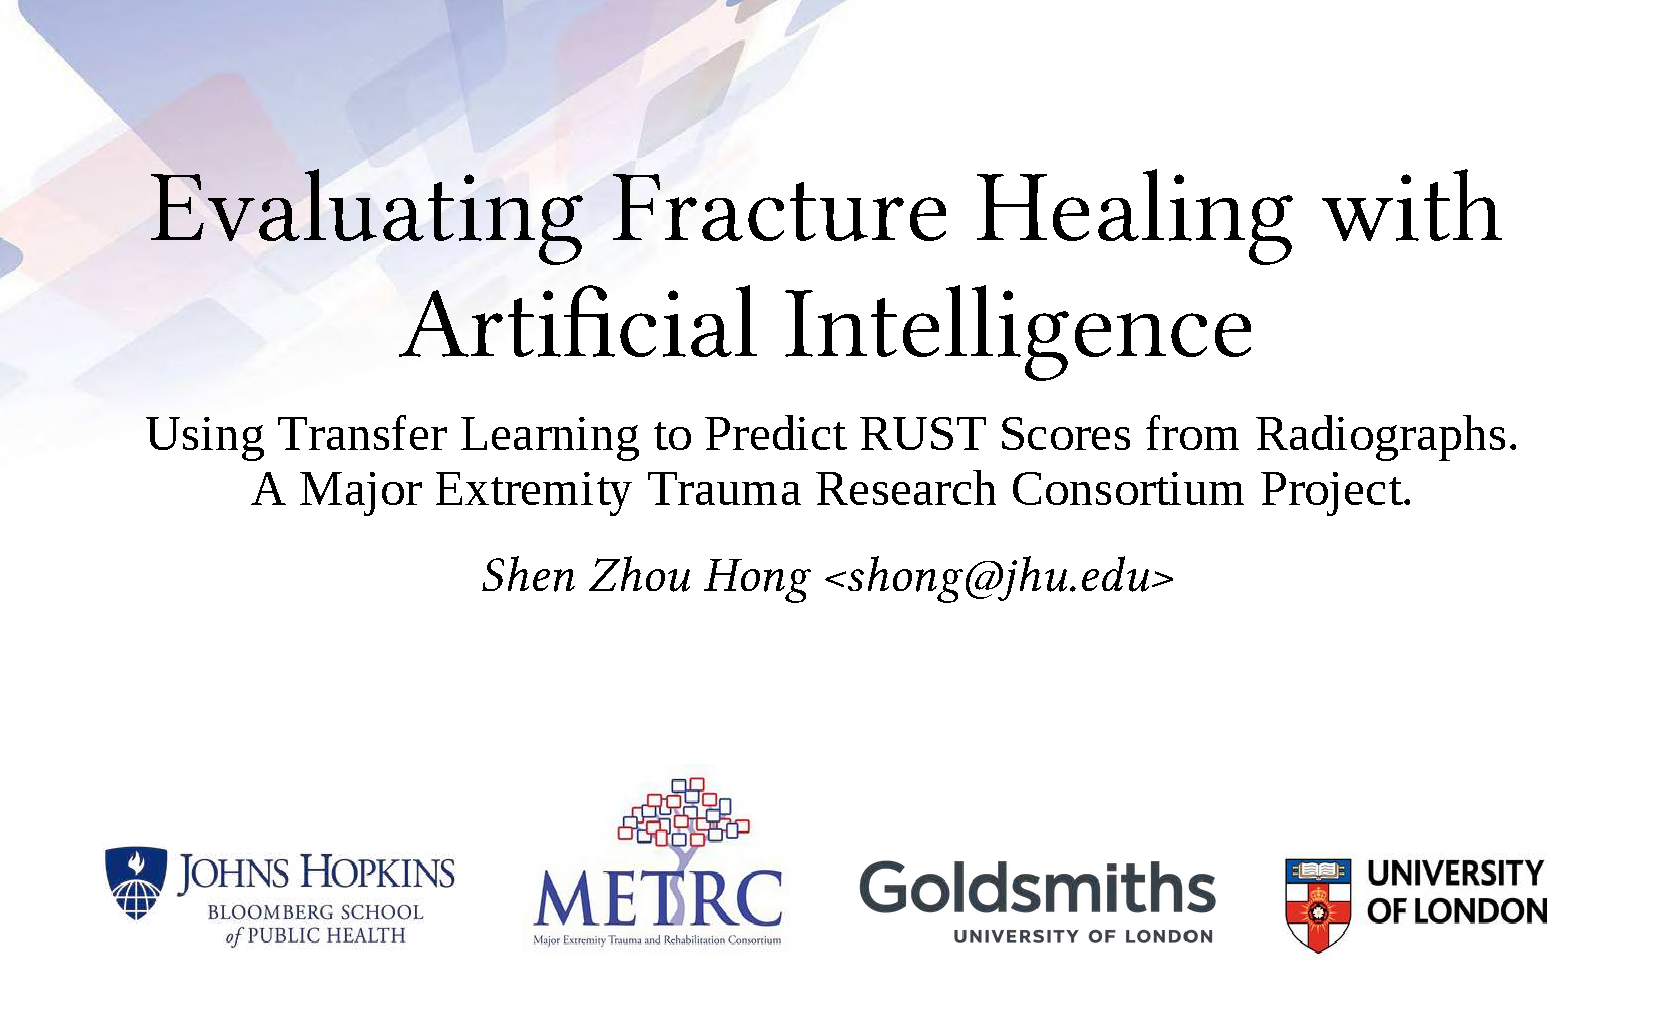
\includegraphics[
page=1,
width=\textwidth,
angle=0,
right
]{media/metrc-ai-presentation.pdf}

% Include the remaining slides as minipages of groups of two
\foreach \n in {2,4,6,8,10,12,14,16,18,20}{
    \begin{minipage}{.49\textwidth}%
        \includegraphics[
            page=\n,
            width=\textwidth,
            angle=0,
            right
        ]{media/metrc-ai-presentation.pdf}
    \end{minipage}%
    \begin{minipage}{.49\textwidth}%
        \includegraphics[
            page=\the\numexpr\n+1\relax,
            width=\textwidth,
            angle=0,
            right
        ]{media/metrc-ai-presentation.pdf}
    \end{minipage}

    \vfill
}
}

\setlength{\headwidth}{\textwidth}
{
\setlength{\parindent}{0pt}
\section{Poster Presentation}
Final project poster presentation, given on 2023-05-11 at Goldsmiths College, University of London.

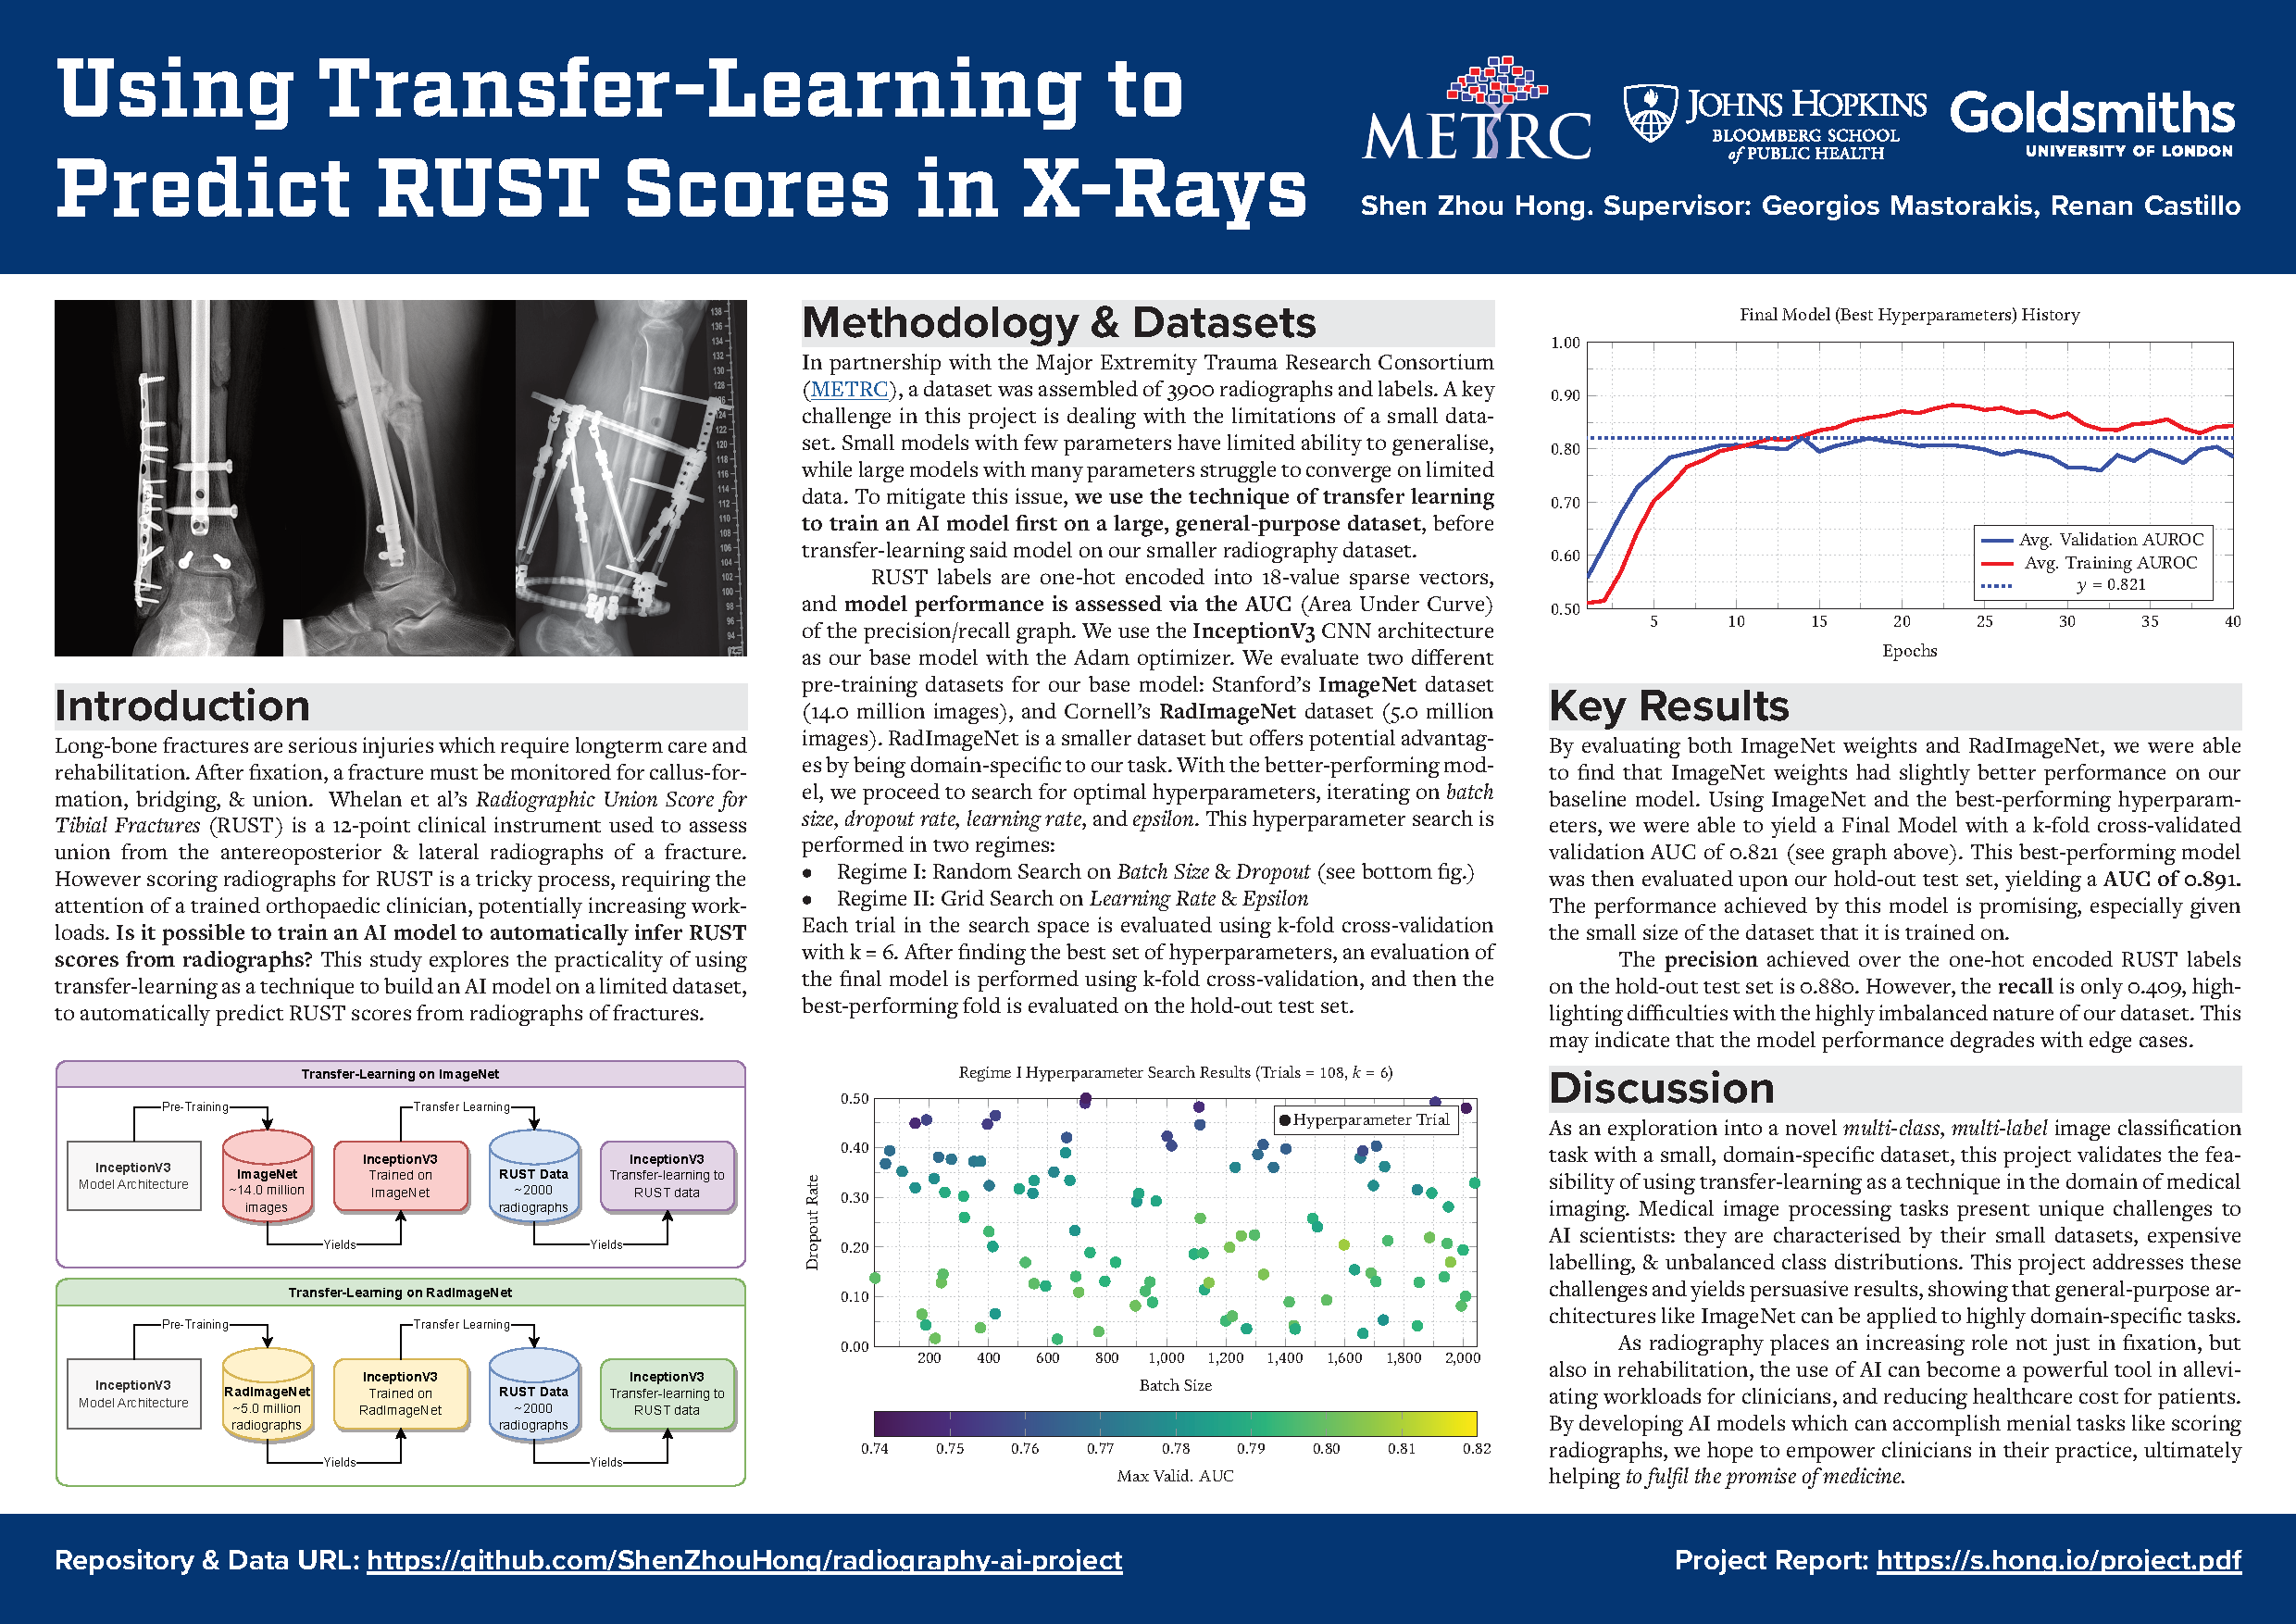
\includegraphics[
    height=0.9\textwidth,
    angle=90,
    center
]{media/poster.pdf}
}

\backmatter

\newgeometry{
    textwidth=0.8\paperwidth,
    textheight=0.8\paperheight,
}
\setlength{\headwidth}{\textwidth}

% Print every citation in citations.bib, even if unused by \autocite
% \nocite{*}

\chapter{Bibliography}

\printbibliography[env=ieee-protrusion, heading=none]

\end{document}
